%!TEX program = xelatex
% !Mode:: "TeX:UTF-8"

\def\xuewei{Doctor} % 定义学位 Doctor or Master
\documentclass[cs4size,openany,oneside,UTF8,nofonts,AutoFakeBold]{ctexbook}
\usepackage[a4paper,text={160true mm,234true mm},top=30.5true mm,left=25true mm,head=5true mm,headsep=2.5true mm,foot=8.5true mm]{geometry}
\usepackage{ccaption}
\usepackage{booktabs}
\usepackage{longtable}
\usepackage{caption}
\usepackage{amsmath}
\usepackage{amssymb}
\usepackage{mathtools}
\usepackage{bigints}
\usepackage{bm}
\usepackage{txfonts}
\usepackage{graphicx}
\usepackage{enumitem}
\usepackage{fancyhdr}
\usepackage{ntheorem}
\usepackage{titlesec}
\usepackage{titletoc}                   % 控制目录的宏包
\usepackage{subfigure}
\usepackage{tabularx}
\usepackage[sort&compress,numbers]{natbib}
\usepackage[boxed,linesnumbered,algochapter]{algorithm2e}	
\usepackage{listings}
\lstset{ columns=flexible, breaklines=true }

\usepackage{tikz-dependency}
\usepackage{multirow}
\usepackage{url}

\usepackage[xetex,
            bookmarksnumbered=true,
            bookmarksopen=true,
            colorlinks=false,
            pdfborder={0 0 1},
            citecolor=blue,
            linkcolor=red,
            anchorcolor=green,
            urlcolor=blue,
            breaklinks=true,
            naturalnames  %与algorithm2e宏包协调
            ]{hyperref}
\defaultfontfeatures{Mapping=tex-text}
\xeCJKsetemboldenfactor{1}%只对随后定义的CJK字体有效
\setCJKfamilyfont{hei}{SimHei}
\xeCJKsetemboldenfactor{4}
\setCJKfamilyfont{song}{SimSun}
\xeCJKsetemboldenfactor{1}
\setCJKfamilyfont{fs}{FangSong}
\setCJKfamilyfont{kai}{KaiTi}
\setCJKfamilyfont{li}{LiSu}
\setCJKfamilyfont{xw}{STXinwei}
\setCJKmainfont{SimSun}
\setCJKsansfont{SimHei}
\setmainfont{Times New Roman}
\setsansfont{Arial}
\newcommand{\heiti}{\CJKfamily{hei}}% 黑体   (Windows自带simhei.ttf)
\newcommand{\songti}{\CJKfamily{song}}    % 宋体   (Windows自带simsun.ttf)
\newcommand{\fs}{\CJKfamily{fs}}        % 仿宋体 (Windows自带simfs.ttf)
\newcommand{\kaishu}{\CJKfamily{kai}}      % 楷体   (Windows自带simkai.ttf)
\newcommand{\li}{\CJKfamily{li}}        % 隶书   (Windows自带simli.ttf)
\newcommand{\xw}{\CJKfamily{xw}}        % 隶书   (Windows自带simli.ttf)
\newfontfamily\arial{Arial}
\newfontfamily\timesnewroman{Times New Roman}


\newcommand{\yihao}{\fontsize{26pt}{26pt}\selectfont}       % 一号, 1.倍行距
\newcommand{\xiaoyi}{\fontsize{24pt}{24pt}\selectfont}      % 小一, 1.倍行距
\newcommand{\erhao}{\fontsize{22pt}{1.25\baselineskip}\selectfont}       % 二号, 1.倍行距
\newcommand{\xiaoer}{\fontsize{18pt}{18pt}\selectfont}      % 小二, 单倍行距
\newcommand{\sanhao}{\fontsize{16pt}{16pt}\selectfont}      % 三号, 1.倍行距
\newcommand{\xiaosan}{\fontsize{15pt}{15pt}\selectfont}     % 小三, 1.倍行距
\newcommand{\sihao}{\fontsize{14pt}{14pt}\selectfont}       % 四号, 1.0倍行距
\newcommand{\xiaosi}{\fontsize{12pt}{12pt}\selectfont}      % 小四, 1.倍行距
\newcommand{\wuhao}{\fontsize{10.5pt}{10.5pt}\selectfont}   % 五号, 单倍行距
\newcommand{\xiaowu}{\fontsize{9pt}{9pt}\selectfont}        % 小五, 单倍行距

\newcommand\litem[1]{\item{\heiti#1\hspace{1.5em}}}

\newenvironment{listitem}{\begin{enumerate}[label={(\arabic*)},itemindent=2em]}{\end{enumerate}}

\usepackage[boxed,linesnumbered,algochapter]{algorithm2e}  % 算法的宏包,注意宏包兼容性,先后顺序为float、hyperref、algorithm(2e),否则无法生成算法列表
\renewcommand{\algorithmcfname}{算法}

%\usepackage{tikz,mathpazo}
%\usetikzlibrary{shapes.geometric, arrows}

\newcommand{\citeayu}[1]{\citeauthor{#1}~(\citeyear{#1})\citeup{#1}}
\newcommand{\citeyqy}[1]{~(\citeyear{#1})\citeup{#1}}

\begin{document}

\titleformat{\chapter}{\center\xiaoer\hei}{\chaptertitlename}{0em}{}
\titlespacing{\chapter}{0pt}{0.5\bseieskip}{0.5\bseieskip}
\titleformat{\section}{\xiaosan\hei}{\thesection}{0em}{}
\titlespacing{\section}{0pt}{0.5\bseieskip}{0.5\bseieskip}
\titleformat{\subsection}{\sihao\hei}{\thesubsection}{0em}{}
\titlespacing{\subsection}{0pt}{0.5\bseieskip}{0.5\bseieskip}
\titleformat{\subsubsection}{\xiaosi\hei}{\thesubsubsection}{0em}{}
\titlespacing{\subsubsection}{0pt}{0pt}{0pt}

\newif\ifxueweidoctor
\newif\ifxueweimaster
\def\temp{Doctor}
\ifx\temp\xuewei
  \xueweidoctortrue  \xueweimasterfalse
\fi
\def\temp{Master}
\ifx\temp\xuewei
  \xueweidoctorfalse  \xueweimastertrue
\fi

% !Mode:: "TeX:UTF-8" 
\setlength{\subfigbottomskip}{0pt}
\CTEXoptions[bibname={主要参考文献}]
\CTEXsetup[name={,},number={}]{chapter}
\captionsetup{labelsep=space,font=small,justification=centering}
\arraycolsep=1.7pt
\graphicspath{{figures/}}
\renewcommand{\subcapsize}{\zihao{5}}
\renewcommand{\thesubfigure}{\alph{subfigure})}
\setcounter{secnumdepth}{4}
\newcommand{\pozhehao}{\raisebox{0.1em}{------}}
\titleformat{\chapter}{\center\zihao{-2}\heiti}{\chaptertitlename}{0.5em}{}
\titlespacing{\chapter}{0pt}{-4.5mm}{8mm}
\titleformat{\section}{\zihao{-3}\heiti}{\thesection}{0.5em}{}
\titlespacing{\section}{0pt}{4.5mm}{4.5mm}
\titleformat{\subsection}{\zihao{4}\heiti}{\thesubsection}{0.5em}{}
\titlespacing{\subsection}{0pt}{4mm}{4mm}
\titleformat{\subsubsection}{\zihao{-4}\heiti}{\thesubsubsection}{0.5em}{}
\titlespacing{\subsubsection}{0pt}{0pt}{0pt}
\makeatletter
\renewcommand\thesection{\@arabic \c@section} % 前面不带 thechapter
\makeatother

\theoremstyle{plain}
\theorembodyfont{\songti\rmfamily}
\theoremheaderfont{\heiti\rmfamily}
\newtheorem{definition}{\heiti 定义}
\newtheorem{example}{\heiti 例}
\newtheorem{algo}{\heiti 算法}
\newtheorem{theorem}{\heiti 定理}
\newtheorem{axiom}{\heiti 公理}
\newtheorem{proposition}{\heiti 命题}
\newtheorem{lemma}{\heiti 引理}
\newtheorem{corollary}{\heiti 推论}
\newtheorem{remark}{\heiti 注解}
\newenvironment{proof}{\noindent{\heiti 证明:}}{\hfill $ \square $ \vskip 4mm}
\theoremsymbol{$\square$}

% 定义页眉和页脚 使用fancyhdr 宏包
\newcommand{\makeheadrule}{
\rule[7pt]{\textwidth}{0.75pt} \\[-23pt]
\rule{\textwidth}{2.25pt}}
\renewcommand{\headrule}{
    {\if@fancyplain\let\headrulewidth\plainheadrulewidth\fi
     \makeheadrule}}
\makeatother
		
\pagestyle{fancyplain}
\renewcommand{\chaptermark}[1]{\relax}
\renewcommand{\sectionmark}[1]{\markright{#1}}
\fancyhf{}
\ifxueweidoctor
  \fancyhead[CO]{\songti \zihao{-5}\rightmark}
  \fancyhead[CE]{\songti \zihao{-5} 哈尔滨工业大学博士学位论文开题报告}%
  \fancyfoot[C]{\zihao{-5} -~\thepage~-}
	\renewcommand\bibsection{\section*{\centerline{\bibname}}
	\markboth{哈尔滨工业大学博士学位论文开题报告}{\bibname}}
\fi
\ifxueweimaster
  \fancyhead[C]{\songti \zihao{-5} 哈尔滨工业大学硕士学位论文开题报告}
  \fancyfoot[C]{\zihao{-5} -~\thepage~-}
	\renewcommand\bibsection{\section*{\centerline{\bibname}}
	\markboth{哈尔滨工业大学硕士学位论文开题报告}{\bibname}}
\fi

\renewcommand{\CJKglue}{\hskip 0.56pt plus 0.08\baselineskip} %加大字间距,使每行33个字
\def\defaultfont{\renewcommand{\baselinestretch}{1.62}\normalsize\selectfont}
% 调整罗列环境的布局
\setitemize{leftmargin=3em,itemsep=0em,partopsep=0em,parsep=0em,topsep=-0em}
\setenumerate{leftmargin=3em,itemsep=0em,partopsep=0em,parsep=0em,topsep=0em}
\renewcommand{\theequation}{\arabic{equation}}
\renewcommand{\thetable}{\arabic{table}}
\renewcommand{\thefigure}{\arabic{figure}}

\makeatletter
\renewcommand{\p@subfigure}{\thefigure~}
\makeatother

\newcommand{\citeup}[1]{\textsuperscript{\cite{#1}}} % for WinEdt users

% 封面、摘要、版权、致谢格式定义
\makeatletter
\def\title#1{\def\@title{#1}}\def\@title{}
\def\titlesec#1{\def\@titlesec{& \rule[-4pt]{200pt}{1pt}\hspace{-326pt}\centerline{\textbf{#1}}}}\def\@titlesec{}
\def\affil#1{\def\@affil{#1}}\def\@affil{}
\def\subject#1{\def\@subject{#1}}\def\@subject{}
\def\author#1{\def\@author{#1}}\def\@author{}
\def\bdate#1{\def\@bdate{#1}}\def\@bdate{}
\def\supervisor#1{\def\@supervisor{#1}}\def\@supervisor{}
\def\assosupervisor#1{\def\@assosupervisor{\textbf{副\hfill 导\hfill 师} & \rule[-4pt]{200pt}{1pt}\hspace{-326pt}\centerline{\textbf {#1}}\\}}\def\@assosupervisor{}
\def\cosupervisor#1{\def\@cosupervisor{\textbf{联\hfill 合\hfill 导\hfill 师} & \rule[-4pt]{200pt}{1pt}\hspace{-326pt}\centerline{\textbf {#1}}\\}}\def\@cosupervisor{}
\def\date#1{\def\@date{#1}}\def\@date{}
\def\stuno#1{\def\@stuno{#1}}\def\@stuno{}
% 定义封面
\ifxueweidoctor
\def\makecover{
    \thispagestyle{empty}
    \zihao{-2}\vspace*{10mm}
		\renewcommand{\CJKglue}{\hskip 2pt plus 0.08\baselineskip}
    \centerline{\heiti\textbf{哈尔滨工业大学}}
		\vspace{10mm}
		\centerline{\zihao{2}\songti\textbf{博士学位论文开题报告}}
    \zihao{-2}\vspace*{10mm}
		\renewcommand{\CJKglue}{\hskip 2pt plus 0.08\baselineskip}
    \centerline{\songti\textbf{题目:\textbf\@title}}
		\renewcommand{\CJKglue}{\hskip 0pt plus 0.08\baselineskip}
    \zihao{3}\vspace{4\baselineskip}
    \hspace*{36pt}{\songti
	\renewcommand{\arraystretch}{1.3}
    \begin{tabular}{l@{}l}
    \textbf{院\hfill (系)}   & \rule[-4pt]{200pt}{1pt}\hspace{-326pt}\centerline{\textbf\@affil}\\
    \textbf{学\hfill 科}     & \rule[-4pt]{200pt}{1pt}\hspace{-326pt}\centerline{\textbf\@subject}\\
    \textbf{导\hfill 师}     & \rule[-4pt]{200pt}{1pt}\hspace{-326pt}\centerline{\textbf\@supervisor}\\
    \textbf{研\hfill 究\hfill 生}      & \rule[-4pt]{200pt}{1pt}\hspace{-326pt}\centerline{\textbf\@author}\\
    \textbf{学\hfill 号}  & \rule[-4pt]{200pt}{1pt}\hspace{-326pt}\centerline{\textbf\@stuno}\\
    \textbf{开题报告日期} & \rule[-4pt]{200pt}{1pt}\hspace{-326pt}\centerline{\textbf\@date}\\
    \end{tabular}\renewcommand{\arraystretch}{1}}
	\vfill
    \centerline{\songti\textbf{研究生院制}}
    \vspace{0.5\baselineskip}
    \centerline{\songti\textbf{二〇一四年九月}}

%%定义内封
    %%新版本没有内封
%\newpage
%\thispagestyle{empty}
%\zihao{5}\vspace*{2em}
%\begin{center}
%  \heiti\zihao{3}说\hspace{3em}明
%\end{center}
%\vspace*{40pt}
%	\renewcommand{\arraystretch}{1.25}
%    {\songti\zihao{5}
%    \hangindent=2em\noindent 一、开题报告应包括下列主要内容:
%    \begin{enumerate}[leftmargin=36pt]
%    \item 课题来源及研究的目的和意义;
%    \item 国内外在该方向的研究现状及分析(文献综述);
%    \item 前期的理论研究与试验论证工作的结果;
%    \item 学位论文的主要研究内容、实施方案及其可行性论证;
%    \item 论文进度安排,预期达到的目标;
%    \item 为完成课题已具备和所需的条件、外协计划及经费;
%    \item 预计研究过程中可能遇到的困难、问题,以及解决的途径;
%    \item 主要参考文献(应在~50~篇以上,其中外文资料不少于二分之一,参考文献中近五年内发表的文献一般不少于三分之一,且必须有近二年内发表的文献资料)。
%    \end{enumerate}
%    \noindent 二、开题报告字数应不少于~1.5~万字。
%
%    \noindent 三、开题报告时间应最迟应于第四学期结束前完成。
%
%    \hangindent=2em\noindent 四、若本次开题报告未通过,需在三个月内再次进行开题报告。第二次学位论文开题报告
%    仍未通过者,将取消其学籍。
%
%    \hangindent=2em\noindent 五、开题报告结束后,评议小组要填写《博士学位论文开题报告评议结果》上报院(系)研
%    究生教学秘书备案。
%
%    \noindent 六、此表不够填写时,可另加附页。
%    }
%	\renewcommand{\arraystretch}{1}
    \clearpage
}
\fi

\ifxueweimaster
\def\makecover{
    \thispagestyle{empty}
    \zihao{-2}\vspace*{10mm}
		\renewcommand{\CJKglue}{\hskip 2pt plus 0.08\baselineskip}
    \centerline{\kaishu\textbf{哈尔滨工业大学}}
		
		\vspace{10mm}
		\centerline{\zihao{2}\songti\textbf{硕士学位论文开题报告}}

		\renewcommand{\CJKglue}{\hskip 0pt plus 0.08\baselineskip}
\vspace{30pt}
\zihao{-2}
\begin{center}\songti\textbf{题~目:\@title}\end{center}
\vspace{30pt}
    \zihao{3}
    \hspace*{68pt}{\songti
	\renewcommand{\arraystretch}{1.3}
    \begin{tabular}{l@{}l}
    \textbf{院\hfill (系)}   & \rule[-4pt]{200pt}{1pt}\hspace{-326pt}\centerline{\textbf\@affil}\\
    \textbf{学\hfill 科}     & \rule[-4pt]{200pt}{1pt}\hspace{-326pt}\centerline{\textbf\@subject}\\
    \textbf{导\hfill 师}     & \rule[-4pt]{200pt}{1pt}\hspace{-326pt}\centerline{\textbf\@supervisor}\\
    \@assosupervisor
	\@cosupervisor
    \textbf{研\hfill 究\hfill 生}      & \rule[-4pt]{200pt}{1pt}\hspace{-326pt}\centerline{\textbf\@author}\\
    \textbf{学\hfill 号}  & \rule[-4pt]{200pt}{1pt}\hspace{-326pt}\centerline{\textbf\@stuno}\\
    \textbf{开题报告日期} & \rule[-4pt]{200pt}{1pt}\hspace{-326pt}\centerline{\textbf\@date}\\
    \end{tabular}
		\renewcommand{\arraystretch}{1}}
	\vfill
    \centerline{\songti\textbf{研究生院培养处制}}

%%定义内封
\newpage
\thispagestyle{empty}
\zihao{5}\vspace*{2em}
\begin{center}
  \heiti\zihao{3}说\hspace{3em}明
\end{center}
\vspace*{40pt}
	\renewcommand{\arraystretch}{1.25}
    {\songti\zihao{5}
    \hangindent=2em
	\noindent 一、开题报告应包括下列主要内容:
    \begin{enumerate}[leftmargin=36pt]
	\item 课题来源及研究的目的和意义;
	\item 国内外在该方向的研究现状及分析;
	\item 主要研究内容;
	\item 研究方案及进度安排,预期达到的目标;
	\item 为完成课题已具备和所需的条件和经费;
	\item 预计研究过程中可能遇到的困难和问题,以及解决的措施;
	\item 主要参考文献。
    \end{enumerate}
    \noindent 二、对开题报告的要求
	\begin{enumerate}[leftmargin=36pt]
	\item 开题报告的字数应在~5000~字以上;
	\item 阅读的主要参考文献应在~20~篇以上,其中外文资料应不少于三分之一。硕士研究生应在导师的指导下着重查阅近年内发表的中、\hspace{-1pt}外文期刊文章。\hspace{-1pt}本学科的基础和专业课教材一般不应列为参考资料。
    \end{enumerate}
    \noindent 三、开题报告时间应最迟不得超过第三学期的第三周末。

    \hangindent=2em\noindent 四、如硕士生首次开题报告未通过,\hspace{-2pt}需在一个月内再进行一次。\hspace{-3pt}若仍不通过,\hspace{-2pt}则停止硕士论文工作。

    \noindent 五、此表不够填写时,可另加附页。

\hangindent=2em\noindent 六、开题报告进行后,此表同硕士学位论文开题报告评议结果存各系(院)研究生秘书书处,以备研究生院及所属学院进行检查。

    }
	\renewcommand{\arraystretch}{1}
    \clearpage
}
\fi
\makeatother

% !Mode:: "TeX:UTF-8"

\affil{机电工程学院}
\subject{机械制造及其自动化}
\author{于冬梅}
\supervisor{某某某教授}
\assosupervisor{副导名}%若无副导师,请屏蔽掉此句
\cosupervisor{联导名}%若无联合导师,请屏蔽掉此句
\date{2011年7月20日}
\stuno{09S906001}
\bdate{2009年9月}

\ifxueweidoctor
  \title{局部多孔质气体静压轴承} %论文题目,此处最多12个字,题目剩余的字放在\ctitlesec里面
  \titlesec{关键技术的研究}
\fi
\ifxueweimaster
  \title{局部多孔质气体静压轴承关键技术的研究}
\fi

\makecover
\clearpage
\setcounter{page}{1} 
\zihao{-4}
\tableofcontents    % 中文目录
\chapter*{中文语义依存图分析技术研究}
%\animategraphics[height=2.8in,autoplay,loop,controls]{12}{animate_}{0}{22}

\section{课题来源及研究的目的和意义}

让机器理解自然语言(Natural Language Understanding, NLU),是自然语言处理(Natural Language Processing, NLP)领域最根本也是最重要的问题之一。要实现在语义层面上理解自然语言,一般来说需要对原始文本自底向上进行分词、词性标注、命名实体识别、句法分析,最后才能进行语义分析。

然而,由于中文严重缺乏形态变化,词类与句法成分没有严格的对应关系,导致中文句法分析的精度始终不高。例如,在英文宾州句法树库(Penn Treebank, PTB)上目前句法分析准确率已经能达到95\%,而在中文宾州句法树库(Chinese Penn Treebank, CTB)上则只能达到88\% \citeyqy{dozat2017deep}。为了解决这些问题,哈工大社会计算与信息检索研究中心(HIT-SCIR)结合中文重意合、在形式分析上有劣势的语言特点,于2011年在世界上最早提出了跨越句法分析直接进行语义依存分析的思路,并与北京语言大学合作标注了中文语义依存树语料库,用树结构融合依存结构和语义关系。此后又将其扩展为语义依存图,从而更全面地刻画句中词之间的语义关系。

语义依存分析(Semantic Dependency Parsing)是通往语义深层理解的一条蹊径,它通过在句子结构中分析实词间的语义关系来回答句子中“Who did what to whom when and where”等问题。以图~\ref{fig:sdp0}中的中文句子“张三前天告诉李四一件事”为例,通过语义依存分析,我们能获知“谁告诉李四一件事?”、“张三告诉谁一件事?”、“张三何时告诉李四一件事?”及“张三告诉李四什么?”等问题的答案。

\begin{figure}[tb]
	\begin{center}
		\begin{small}
			\begin{dependency}[arc edge, arc angle=80, text only label, label style={above}]
				\begin{deptext} [row sep=0.4cm, column sep=.1cm]
					\ ROOT$_0$ \& 张三 $_1$ \& 前天$_2$ \& 告诉$_3$ \&  李四$_4$  \& 一件$_5$ \& 事$_6$ \\
				\end{deptext}
				\depedge[edge style={black,thick}]{1}{4}{\color{black}Root}
				\depedge[edge style={black,thick}]{4}{2}{\color{black}Agt}
				\depedge[edge style={black,thick}]{4}{3}{\color{black}Time}
				\depedge[edge style={black,thick}]{4}{5}{\color{black}Datv}
				\depedge[edge style={black,thick}]{4}{7}{\color{black}Cont}
				\depedge[edge style={black,thick}]{7}{6}{\color{black}Cont}
			\end{dependency}
			\caption{语义依存表示示例}\label{fig:sdp0}
		\end{small}
	\end{center}
\end{figure}

\begin{figure}[tb]
	\begin{center}
		\begin{small}
			\begin{dependency}[arc edge, arc angle=80, text only label, label style={above}]
				\begin{deptext} [row sep=0.4cm, column sep=.1cm]
					\ ROOT$_0$ \& 前天$_1$ \& ,$_2$ \& 张三$_3$ \&  将$_4$  \& 一件$_5$ \& 事$_6$ \& 告诉$_7$ \& 李四$_8$  \\
				\end{deptext}
				\depedge[edge style={black,thick}]{1}{8}{\color{black}Root}
				\depedge[edge style={black,thick}]{2}{3}{\color{black}mPunc}
				\depedge[edge style={black,thick}]{7}{5}{\color{black}mPrep}
				\depedge[edge style={black,thick}]{7}{6}{\color{black}Quan}
				\depedge[edge style={black,thick}]{8}{2}{\color{black}Time}
				\depedge[edge style={black,thick}]{8}{4}{\color{black}Agt}
				\depedge[edge style={black,thick}]{8}{7}{\color{black}Cont}
				\depedge[edge style={black,thick}]{8}{9}{\color{black}Datv}
			\end{dependency}
			\caption{语义依存表示示例}\label{fig:sdp1}
		\end{small}
	\end{center}
\end{figure}

\begin{figure}[tb]
	\begin{center}
		\begin{small}
			\begin{dependency}[arc edge, arc angle=80, text only label, label style={above}]
				\begin{deptext} [row sep=0.6cm, column sep=.5cm]
					\ ROOT$_0$ \& 早起 $_1$ \& 使$_2$ \& 人$_3$ \&  健康$_4$ \\
				\end{deptext}
				\depedge[edge style={black,thick}]{1}{3}{\color{black}Root}
				\depedge[edge style={black,thick}]{3}{2}{\color{black}Exp}
				\depedge[edge style={black,thick}]{3}{4}{\color{black}Datv}
				\depedge[edge style={black,thick}]{3}{5}{\color{black}eResu}
				\depedge[edge style={black,thick}]{5}{4}{\color{black}Exp}
			\end{dependency}
			\caption{语义依存图表示示例}\label{fig:sdg0}
		\end{small}
	\end{center}
\end{figure}

此外,与句法分析不同,语义分析可以跨越句子的表层结构直接获取深层语义表达的本质,例如图~\ref{fig:sdp1}中的句子“昨天,张三将一个秘密告诉李四。”虽然与图~\ref{fig:sdp0}中的句子表述形式不同,但含义相同,因此它们的语义依存结构相同。因此语义依存分析能为机器翻译、问答系统、对话生成等对语义信息要求较高的下游任务提供很大帮助。

语义依存分析建立在依存理论基础上,是对语义的深层分析,具有形式简洁,易于理解和运用的优势。具体可分为两个阶段,首先是根据依存语法建立依存结构,即找出句子中的所有修饰词与核心词对,然后再对所有的修饰词与核心词对指定语义关系。因此,语义依存分析可以同时描述句子的结构和语义信息。

与分词、词性标注、句法依存分析等历史悠久的研究课题相比,语义依存分析算得上是一个新兴课题。由于其与句法依存分析在结构上的相似之处,语义依存树的分析基本可以沿用已经有诸多成果的句法依存分析领域的方法。然而近年来人们发现树结构已经无法胜任刻画句子中复杂的语义关系的任务,研究者们逐渐将目光聚集到约束更少的图结构上,希望用图结构来表示这些语义关系。因此,无论在中文还是在以英文为代表的一些外语中,越来越多图结构的语义依存语料库应运而生。例如图~\ref{fig:sdg0}的句子“早起使人健康”中,“人”同时作为“使”的与事者(Dative, Datv)和“健康”的当事者(Experiencer, Exp)。

图结构在带来更全面的语义表示的同时,也给语义依存分析任务带来了巨大的挑战。对于原来的依存树结构,每个词只有一个父节点,而在依存图中,每个词可能有多个父节点,这就给分析系统带来了很大的不确定性,从而增加了语义依存分析任务的难度。因此,本学位论文的研究目标集中在图结构的中文语义依存分析上,希望能通过实现更好的语义依存分析器,提高中文语义依存分析的精度,为下游任务提供更好的语义信息,弥补中英文由于语言特性在句法分析领域产生的差距。
% !Mode:: "TeX:UTF-8" 

\section{国内外在该方向的研究现状及分析}
\subsection{国内外研究现状}

语义依存分析是一个新兴课题,虽然已经引起了许多研究者的关注,但是相关的数据集和研究工作相比分词、词性标注等历史悠久的任务都比较有限,而国内的研究更是非常少,因此这里将国内外的研究现状总结到一起描述。

语义依存树与句法依存树主要的区别在于依存弧上的标签不同,这源自于两种任务目标上的区别。因此语义依存树的分析基本可以沿用句法依存分析方法,对于后者目前已经存在大量的研究工作,目前应用最多的主要可以分为两大类:基于转移(Transition-based)和基于图(Graph-based)的依存分析。基于图的算法将依存分析转换为在有向完全图中求解最大生成树的问题,是基于动态规划的一种图搜索算法。该算法由\citeayu{mcdonald-crammer-pereira:2005:ACL}提出,是一种全局最优的搜索算法。\citeayu{yamada2003statistical} 提出的基于转移的依存分析算法将句子的解码过程建模为一个转移序列的构造过程。其依存分析模型的目标是通过学习得到一个能够准确的预测下一步转移动作的分类器。

语义依存图与句法依存树除了上述的依存弧标签不同之外,结构上也有所差异。语义依存图打破了传统的依存树结构,允许多父节点的存在(在依存树中一个词只能有一个父节点),因此能够刻画句中词之间更丰富的语义关系。但多父节点的存在同时也使得对语义依存图的分析更具挑战性。目前对语义依存图的分析工作主要使用的方法都是对上述基于转移和基于图的依存分析方法的扩展。下面我们首先简要介绍目前国内外的语义依存图数据集,然后分别对基于转移和基于图的语义依存图分析工作进行总结。

\subsubsection{语义依存图数据集}

目前国内的语义依存图数据集只有由哈工大社会计算与信息检索研究中心(HIT-SCIR)和北京语言大学合作标注的 SemEval-2016 Task 9 中文语义依存图数据集\citeyqy{che-EtAl:2016:SemEval}。为了解决 SemEval-2012 Task 5 语义依存树数据集\citeyqy{che-EtAl:2012:STARSEM-SEMEVAL}中语义关系彼此易混淆、语义关系数量太大、刻画语义不全面等问题,在中文语义依存图数据集中用依存图结构代替依存树。形式上类似于依存句法结构,但必要时突破树形结构(BH-SDP-v2标注体系)。这样的突破使得对连动、兼语、概念转位等汉语中常见的现象的分析更全面深入,当然这也给依存分析器的构建带来了很大的难度,因为任何词都可能有多个父节点。图~\ref{fig:sem16diff}直观地展示了语义依存树与依存图的区别。

\begin{figure}[tbhp]
	\centering
	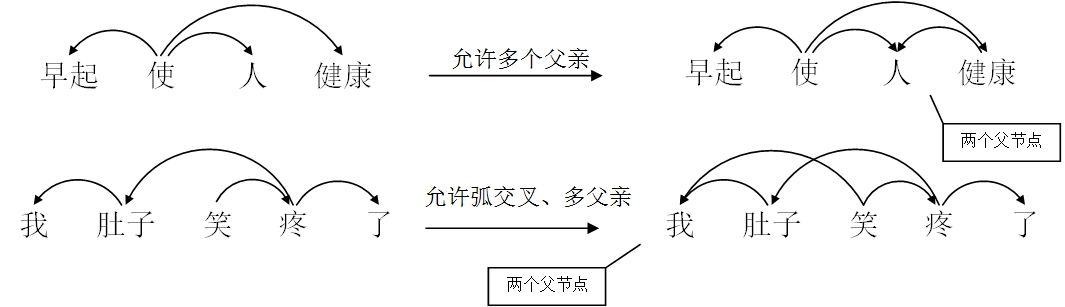
\includegraphics[width=85mm]{picture/sem16diff.jpg}
	\caption{中文语义依存树与语义依存图对比示例}
	\label{fig:sem16diff}
\end{figure}

BH-SDP-v2标注体系压缩了语义关系类型的数量,重新组织并缩减了语义关系,将关系分为主要语义角色、事件关系、关系标记,从而减少不必要的类间关系混淆。语义关系在保留了一般语义关系、反关系基础上,还增加了嵌套关系,用来标记一个事件降级充当了另一个事件的成分。SemEval-2016 Task 9 中文语义依存图数据集中包含10068句新闻语料和15362句课文句子。新闻句子平均长度是31个词,课本句子平均长度是14个词。该数据集被用于 SemEval-2016 Task 9 国际公开评测上。

\begin{figure}[tb]
	\centering
	\small
	\subfigure[DM]{\label{fig:sem15-dm}
		\begin{dependency}[theme = simple,label style={font=\bfseries,thick}]
			\begin{deptext}[column sep=0.3em]
				Last \& week \& , \& shareholders \& took \& their \& money \& and \& ran \\
			\end{deptext}
			\deproot[edge unit distance=2.8ex]{5}{top}
			\depedge{1}{2}{arg1}
			\depedge{2}{5}{loc}
			\depedge{5}{4}{arg1}
			\depedge{5}{7}{arg2}
			\depedge{5}{9}{\_and\_c}
			\depedge{6}{7}{poss}
			\depedge[edge start x offset = 6pt]{9}{4}{arg1}
			%\depedge[edge start x offset=-4pt, edge end x offset=-3pt]{8}{9}{conj}
		\end{dependency}
	}
	
	\subfigure[PAS]{\label{fig:sem15-pas}
		\begin{dependency}[theme = simple,label style={font=\bfseries,thick}]
			\begin{deptext}[column sep=0.3em]
				Last \& week \& , \& shareholders \& took \& their \& money \& and \& ran \\
			\end{deptext}
			\deproot[edge unit distance=2.8ex]{8}{top}
			\depedge{1}{2}{arg1}
			\depedge{2}{8}{arg1}
			\depedge{5}{4}{arg1}
			\depedge{5}{7}{arg2}
			\depedge{6}{7}{arg1}
			\depedge{8}{5}{coord}
			\depedge{8}{9}{coord}
			\depedge[edge start x offset = 6pt]{9}{4}{arg1}
		\end{dependency}
	}
	
	\subfigure[PSD]{\label{fig:sem15-psd}
		\begin{dependency}[theme = simple,label style={font=\bfseries,thick}]
			\begin{deptext}[column sep=0.3em]
				Last \& week \& , \& shareholders \& took \& their \& money \& and \& ran \\
			\end{deptext}
			\deproot[edge unit distance=2.8ex]{5}{top}
			\deproot[edge unit distance=2.8ex]{9}{top}
			\depedge{2}{1}{rstr}
			\depedge{5}{2}{twhen}
			\depedge{5}{4}{act}
			\depedge{5}{7}{pat}
			\depedge{7}{6}{app}
			\depedge{8}{5}{conj}
			\depedge[edge start x offset=-4pt, edge end x offset=-3pt]{8}{9}{conj}
			\depedge[edge start x offset=3pt]{9}{4}{act}
			\depedge[edge start x offset=3pt]{9}{2}{twhen}
		\end{dependency}
	}
	\caption{广义语义依存图三种标注体系示例}
	\label{fig:sem15}
	
\end{figure}

国外的语义依存图数据集主要是SemEval-2015 Task 18广义(Broad-Coverage)语义依存图数据集。
其目标是获取句子内部所有实词之间的谓词论元关系,即获取表示该句子含义的语义结构。构建该数据库的目的是寻找更具普适性的图结构,从而提供对“Who did what to whom”等问题更直接的分析方式。
该语料库中使用了三种不同的标注体系(图~\ref{fig:sem15}给出了三种标注的例子),分别是:

\begin{enumerate}
\item \textbf{DM (DELPH-IN MRS-Derived Bi-Lexical Dependencies)}
\ \ \ \ 该语义依存图标注来源于参考LinGO英文资源语法(English Resource Grammar)给出的句法、语义信息进行人工重标注的DeepBank语料。
	
\item \textbf{PAS (Enju Predicate–Argument Structures)}
\ \ \ \ Enju树库和分析器来源于对宾州树库的HPSG形式自动标注。PAS语义依存图是直接从Enju树库中抽取的,没有进行内容转换。
	
\item \textbf{PSD (Prague Semantic Dependencies)}
\ \ \ \ 布拉格捷克语-英语依存树库(Prague Czech-English Dependency Treebank)是包括宾州树库华尔街日报部分及其捷克语翻译的依存树的语料库。PSD语义依存图是从该树库的构造语法标注层(tectogrammatical annotation layer)中抽取出来的。
\end{enumerate} 

该数据集中包括英语、中文和捷克语的语料。其中英语部分来自宾州树库(PTB)华尔街日报和布朗部分,包括35657句训练语料、1410句同领域测试语料及1849句不同领域(来自布朗部分)测试语料,拥有DM、PAS和PSD三种标注规范的语义依存图。中文部分来自中文宾州树库(CTB 7.0),包括31113句训练语料和1670句同领域测试语料,只有PAS规范的标注。捷克语部分来自宾州树库华尔街日报部分的捷克语翻译,包括42076句训练语料、1670句同领域测试语料及5226句不同领域测试语料,只有PSD规范的标注。 
该语料的英语部分首先用于 SemEval-2014 Task 8 评测\citeyqy{oepen-EtAl:2014:SemEval}。此后的 SemEval-2015 Task 18 评测任务\citeyqy{oepen-EtAl:2015:SemEval}中,该语料库又加入了中文和捷克语部分语料。

除此之外,还有一些数据集与语义依存图在结构或内容上有相似之处,包括 CoNLL-2009 数据集\citeyqy{hajivc-EtAl:2009:CoNLL-2009-ST}的语义角色标注(Semantic Role Labeling)部分、CCD(CCG Dependencies)\citeyqy{hockenmaier2007ccgbank}、AMR(Abstract Meaning Representation)数据集\citeyqy{W13-2322}、丹麦语依存树库\citeyqy{kromann2003danish}(DDT)和HPSG树库\citeyqy{miyao2005corpus}等。
其中前两个属于语义角色标注范畴,其目的是找出句中一些谓词与其论元之间的关系,因此该任务一般分为两步,第一步是识别出句中的谓词,第二步才是找到每个谓词对应的论元。这里所说的谓词,一般来说指的是动词和名词。而语义依存分析的目的是找到句中所有词之间的语义关系,对词的种类没有限制,因此不需要进行上述的第一步。从两个任务目的上的不同能够发现,语义依存分析能提供一个句子更全面的语义信息。
AMR属于语义网络(Semantic Network),其中图节点表示的是语义概念,不需要与句中的词一一对应。而语义依存图则用有向弧直接表示的句中词之间的语义关系。此外,AMR目前只有英文数据,在中文上没有与之类似的数据集。
丹麦语依存树库和HPSG树库本质上来说也属于依存句法树库,但由于其中也包含一些图结构的依存句法表示,因此在语义依存图没有提出之前,一些对图结构分析算法的研究是在这些数据集上进行的,这些方法对我们也有一定的启示作用。

\subsubsection{基于转移的分析方法}

在基于转移的依存图分析方向上,\citeayu{sagae2008shift}发表了通过向转移系统中增加新的转移动作实现基于转移的依存图分析的先驱性工作。在传统的基于转移的依存树分析系统中,由于每个词只有一个父节点,因此一旦找到一个词的父节点就要将该词从系统中删除(LEFT-REDUCE和RIGHT-REDUCE动作),Sagae等人在转移系统中加入两个新的生成依存弧的动作(LEFT-ATTACH和RIGHT-ATTACH),只生成依存弧而不删除词,从而实现了多父节点结构的生成。他们在丹麦语依存树库和HPSG树库两个含有图结构的依存句法树库中进行了实验。此后该方向上的研究工作主要都集中在通过修改转移系统处理依存图结构。增加两个新的动作是一个最直观的解决依存图分析问题的方法,但是新增的两个动作只生成依存弧,不改变转移系统状态,在执行这两个动作前后转移系统的状态是基本不变的,这也就导致了从当前状态中提取出的用于预测下个转移动作的特征也是基本相同的,这会影响分类器预测的准确性,从而降低系统的整体性能。
\citeayu{Titov:2009:OGP:1661445.1661696}提出了另一种转移系统,在生成弧的同时不改变系统中的词,而是用独立的REDUCE动作删除已经无用的词,同时利用SWAP动作改变系统中词的顺序。

\citeayu{Zhang:2016:TPD:3030588.3030589} 提出了两种新的转移系统,第一种在线重排序(Online re-ordering)系统与Titov的系统类似,第二种基于双栈的(Two-Stack-Based)系统拥有一个额外的栈,用于保存从正在处理词的栈中暂时移除的词,通过MEM和RECALL两个动作实现向该额外的栈中保存词和从该栈中取词。除了转移系统外,基于转移的依存分析中十分重要的另一个部分就是用于在给定转移状态下预测下一个转移动作的分类器。Zhang等人在实验中也发现如果转移动作集合中存在只生成依存弧而不改变转移系统的动作,会影响分类器准确性。为了解决这一问题,他们将与生成依存弧有关的动作(NO、LEFT和RIGHT,分别表示不生成弧,生成向左或向右的弧)和改变转移状态的动作(SHIFT、REDUCE、SWAP等)两两组合,在最终的系统中使用组合后动作,保证了每个动作都会改变转移系统状态,成功提高了系统性能。

\subsubsection{基于图的分析方法}

在基于图的依存分析方向上,\citeayu{mcdonald2006online}首先提出了利用近似Eisner算法\citeyqy{eisner1996three}解决基于图的依存分析中多父节点的生成的方法。他们首先使用原始Eisner算法生成一个投射树(依存弧存在交叉的树),然后对树中的边逐条替换,替换时允许出现多父节点,保留使整体评分增加的替换,从而生成图结构。McDonald等人也在丹麦语依存树库上进行了实验。这种方法本质上来说只是在传统的依存树分析算法得到的结果的基础上进行后处理,将树结构改成图结构,面对较复杂的图结构依然不能算是一个很好的解决方案。

\citeayu{martins2014priberam,almeida-martins:2015:SemEval}提出了一种利用二阶特征的方法,在单个弧的一阶特征基础上,增加了连续兄弟节点、连续多父节点等二阶特征,使用$AD^3$算法\citeyqy{martins2014ad3}进行解码,实现了依存图的预测。$AD^3$算法是一种基于对偶分解的近似离散优化算法。由于这里采用的分解方式不是以弧为因子的(arc-factored),各结构之间存在重叠,所以需要使用该算法进行解码。与McDonald等人的方法相比,该方法能够直接预测出图结构,而不是通过对依存树的后处理生成依存图。

\citeayu{peng-thomson-smith:2017:Long}利用了广义语义依存图语料库中英语部分有三种不同标注的特点,采用了多任务学习方法,仅用一阶特征就在该数据集上取得了当时最好结果。不仅如此,他们还借鉴了基于图的依存树分析研究中对神经网络的成功应用\citeyqy{TACL885},将句中每个词的词向量输入双向长短时记忆网络(Bidirectional Long-Short Term Memory, Bi-LSTM),用其隐层输出作为每个词的表示,然后利用多层感知器(Multi-Layer Perceptron, MLP)计算每条候选弧的分数。通过这种方法,他们的模型即使不使用多任务学习方法,也有很好的表现。


\subsection{国内外文献综述的简析}
\subsubsection{现有工作的总结及其不足}
\label{drawback}

由于语义依存图的概念才提出不久,中文及其他语言上的语义依存图相关数据集构建工作也是近几年才初步完成,语料有限,目前为止国内外对于语义依存图分析的研究工作还比较少。因此,我们不但调研了专门研究语义依存图分析的工作,也从此前对于句法依存图等图结构分析的研究工作中获取灵感。总的来说,目前基于转移的依存分析方法和基于图的依存分析方法都开辟出了各自对图结构进行分析的道路。

在基于转移的分析方法中,目标依存结构是通过在包括待分析句子信息的转移系统(Transition System)中执行一系列的类似移进、规约的转移动作修改转移状态(转移系统中各部分的状态)来生成的,其最终目的是训练一个给定当前转移状态能够预测出接下来要执行的转移动作的分类器。因此,在这类方法中生成依存图的最大困难来自于每个词的父节点由原来的一个变成了任意多个,导致分类器难以判断何时对一个词进行规约。针对这一问题一般的解决办法是修改转移系统,提出新的转移动作替代或补充原有转移动作,从而增强转移系统的处理能力,使其可以产生依存图结构。因此如何设计或修改转移系统,就成为了基于转移的分析方法中一个十分重要的研究问题。此外,由于这类方法的核心是用于预测转移动作的分类器的训练,而分类器预测的依据则是当前的转移状态,因此如何更好、更快、更全面地获得当前转移状态的信息将其作为分类器的分类依据就成为了这类方法中另一个十分值得研究的问题。

在基于图的分析方法中,首先要将目标分成许多子结构,计算出所有可能的子结构的分数。分解方式有很多种,以一条弧为单位的分解称为一阶分解(first-order factorization),以两条弧一组为单位进行的分解称为二阶分解(second-order factorization)。然后利用动态规划算法计算出总分最大的子结构组合。
当分析目标是依存树时,一般使用最大生成树(Max Spanning Tree)算法。在面对依存图结构时,由于每个词的父节点个数由一个变为任意多个,而依存图又有非投射性(弧之间存在交叉),原来的动态规划算法不再适用,只能对每个子结构进行独立判断。如果使用了多种分解方式,则需要采用$AD^3$算法解决各子结构存在重叠时的解码问题。

上述两类方法中的绝大部分工作都使用了诸如线性模型、最大熵模型、结构化感知器等传统统计学机器学习方法。它们都是通过人工特征工程实现从环境中获取信息的,这样人工设计特征模板不但繁琐,需要该领域的专家知识,而且往往无法涵盖所有的信息,同时,对特征字符串的组合也会耗费大量时间。

近年来,模型融合(Model Ensemble)技术在依存句法分析领域已被证明十分有效,但是目前的模型融合方法不是利用多个不同模型的最终结果进行投票决定最终预测结构,就是对同一模型使用不同的随机初始化种子多次训练然后同时使用这些独立训练的模型进行预测。而且后者仅仅被应用在基于转移的依存分析中,并没有工作将这种模型融合方式应用于基于图的依存分析中。这两种模型融合方式虽然简单有效,但没有利用依存分析任务的特性,仅仅是把其它领域的模型融合方式简单搬运到依存分析领域,缺乏针对性。

作为一个新兴研究课题,中外文的语义依存图语料数量都十分有限,这给语义依存图分析研究的进行和高精度语义依存图分析器的训练都带来了巨大挑战。在这种情况下,更应该充分利用现有多种语言的语料资源,同时利用依存句法分析、语义角色标注等已有大量人工标注数据的相关任务帮助提高语义依存图分析器的精度。\citeayu{peng-thomson-smith:2017:Long}已经在SemEval-2015 Task 18英文广义语义依存图数据集上证明了通过多任务学习方法同时学习该数据集的三种标注体系能够有效提高最终的实验结果。但目前这方面的其它工作十分有限,仍有很大的研究空间。

\subsubsection{有待深入研究的问题}

与分词、句法分析等历史悠久的任务相比,语义依存图分析是一个十分年轻的任务,许多相关研究才刚刚起步,无论是在分析方法本身的研究上,还是在提高分析系统性能、利用多语言及其他任务数据的研究上,都有许多工作可以做。对于分析方法来说,基于转移的和基于图的两类依存图分析方法的研究都刚刚开始,孰优孰劣未有定论,因此这两类方法的研究都很有价值和意义。而在有了依存图分析方法之后,提出适应语义依存图任务特性的方法来提高系统性能则成为最重要的问题。另一方面,由于目前语义依存图语料较少,如何充分利用现有多种语言的语料资源以及依存句法分析、语义角色标注等相关任务的数据也是一个十分有意义的研究方向。因此,未来对于语义依存图分析的研究将集中在以下几个方面:

\begin{enumerate}
\item \textbf{基于转移的分析方法}
\ \ \ \ 在传统基于转移的依存树分析方法基础上,如何提出新的转移系统,解决分类器不知道何时对一个词进行规约的问题,使其能生成依存图结构,是基于转移的依存图分析方法的根本。在此基础上,研究如何使用新的信息抽取方式代替原来低效、繁琐的人工特征工程,从而更好、更快、更全面地获得当前转移状态的信息是十分有意义的
	
\item \textbf{基于图的分析方法}
\ \ \ \ 在基于图的分析方法中,第一步计算每个子结构的分数是至关重要的,因为此后使用解码算法得到的依存图结构完全是依赖于第一步中得出的分数的。所以在基于图的分析方法中如何从句子中获取更全面的信息帮助计算子结构的分数是很值得研究的。
	
\item \textbf{利用模型融合技术提高系统性能}
\ \ \ \ 模型融合已经在许多领域证明是一个简单有效的提高系统性能的方法。现有的在依存分析系统中利用模型融合技术的工作实现的仅仅是简单的最终结果投票融合或者是使用不同的随机初始化种子。这些方法并没有考虑到语义依存分析任务的特性,同时可解释性也不强。因此,如何设计一个符合语义依存分析任务特性,能够融合对不同维度信息进行建模的融合方法,将是十分重要的。
	
\item \textbf{利用多语言、多领域数据}
\ \ \ \ 随着深度学习技术在各领域取得的巨大成功,数据量往往与使用深度学习技术的系统性能成正比。由于语义依存图语料有限,如何充分利用现有多种语言的语料资源以及依存句法分析、语义角色标注等已有大量人工标注语料的相关任务数据也是一个十分有意义的研究方向。
	
\end{enumerate}





% !Mode:: "TeX:UTF-8" 
\section{前期的理论研究与实验论证工作的结果}

本课题相关的理论研究始于2015年9月,在经过深入的调研顺滑理论及与其紧密相关的其它自然语言处理技术的基础上,开始对顺滑任务中存在问题进行三方面的尝试。首先,针对顺滑任务中的长距离依赖问题,我们尝试用LSTM来对句子进行表示,同时,为了避免用LSTM的输出直接进行分类所带来的label偏置问题,我们最终的模型会在LSTM表示的基础上加一个CRF层,最终的LSTM-CRF模型相比于传统的模型和直接用LSTM的输出进行分类的模型相比,取得了更好的性能,该工作已经被CCL2016录用。其次,为了保证得到的顺滑句子的句法完整性,同时充分的利用全局的信息,我们尝试用注意力机制的方法,该方法将顺滑任务转化成一个生成的过程,对原句子进行编码后,直接生成目标句子,该方案取得了非常好的性能,该工作已经被COLING2016录用。最后,针对非顺滑块和顺滑块之间相似性,我们尝试基于转移的方案,我们的方案能很好的建模块之间的联系,同时能充分的利用全局的信息,该方案取得了目前最好的实验结果,该工作已经被EMNLP2017录用。
由于LSTM-CRF模型不属于博士课题的研究点,因此本文将简要介绍以下两项工作。

%(1) Enhancing Neural Disfluency Detection with Hand-Crafted Features. (CCL2016, 已发表)

(1) Transition-Based Disfluency Detection using LSTMs. (EMNLP 2017, 已发表)

(2) A Neural Attention Model for Disfluency Detection. (COLING 2016, 已发表)



%3. A Deep Neural Network for Chinese Zero Pronoun Resolution. (Coling 2016)

\subsection{基于转移的顺滑技术研究}
\subsubsection{实验动机}
传统的方法将顺滑任务看作序列标注问题 \citeyqy{zayats2016disfluency,hough2015recurrent,qian2013disfluency,georgila2009using},为句子中的每一个词分配一个标签,然后根据标签判断是否要将其保留。这类方法取得了不错的结果,但其不能很好的解决长距离依赖问题,而且也没有能力利用块级别的信息。

为了利用块级别的信息, \citeayu{ferguson-durrett-klein:2015:NAACL-HLT}尝试使用semi-CRF模型来解决顺滑问题,并且取得了很好的实验效果。但是semi-CRF由于受到马尔科夫假设的约束,其也只能利用局部的块信息。

还有一些工作  \citeyqy{rasooli2013joint,honnibal2014joint,wu-EtAl:2015:ACL-IJCNLP} 尝试将句法分析和顺滑任务联合起来。这种联合模型的主要优点在于它们可以建模长距离的依赖关系,而且能够很好的利用块级别的信息。然而,它要求训练数据要同时标注句法和顺滑信息,这降低了算法的实用性,同时句法分析的噪声可能会严重影响顺滑任务的性能。

受上述观察的启发,我们使用一种不带句法信息的转移系统来解决顺滑问题\citeyqy{zhang-zhang-fu:2016:P16-1}。我们基于转移的方法通过采用和依存句法类似的解码算法来递增地构建和标记输入句子中的不流畅块。
\subsubsection{背景介绍}
	在背景介绍部分,我们简要说明一下基于转移的句法分析方法和在此基础上扩展而来的句法和顺滑联合方法。一个经典的基于转移的arc-eager句法分析器主要由一个存储正在处理的词的堆栈$\sigma$,一个包含将要被处理的词的缓冲区 $\beta$和一个存储已生成的依存弧的存储器 $A$四部分组成。对于该转移系统,有四种类型的转移动作\citeyqy{nivre2008algorithms}
\begin{itemize}
	\item \textit{Shift} : 将缓冲区的顶端的词压到堆栈中去.
	\item \textit{Reduce} : 弹出堆栈顶端的词.
	\item \textit{LeftArc} : 将堆栈顶端的词弹出堆栈,并将其链接到缓冲区的顶端的词下面,作为其孩子节点.
	\item \textit{RightArc} : 将缓冲区顶端的词弹出,并链接到堆栈顶端的词下面,作为其孩子节点
\end{itemize}
许多基于神经网络的句法分析器都遵循这套转移框架,例如\citeayu{dyer-EtAl:2015:ACL-IJCNLP},他们使用不同的LSTM结构来表示从$\sigma$到$\beta$的信息。

对于顺滑任务来说,输入是自动语音识别(ASR)后的可能带有不流畅块的句子。我们将输入句子的词序列表示为 $w_{1}^{n} = (w_1, . . . , w_n )$。顺滑任务的输出是表示为$D_{1}^{n} = (d_1, . . . , d_n )$的标签序列,其中每个$d_i$代表对应的词$w_i$是否属于不流畅的词。因此,顺滑任务可以被建模为给定词序列 $w_{1}^{n}$,搜索最好的序列$D^*$。
\begin{equation}
D^* = argmax_{D}P(D_1^n|w_1^n)\nonumber
\end{equation}
\citeayu{wu-EtAl:2015:ACL-IJCNLP} 提出了一种句法和顺滑联合模型,其在解码过程中,通过增加一个二值分类动作(BCT)来判断哪些词属于非顺滑的词。
\begin{itemize}
	\item \textit{BCT} : 判断当前的词是否为不流畅词。如果是,将其从buffer中删除,并将其标记为不流畅词。否则就从初始的四种动作中选择一种可能性最大的动作来执行。
\end{itemize}
顺滑和句法任务进行联合的优化,
\begin{equation}
\begin{split}
(D^*, T^*) = argmax_{D,T}\prod_{i=1}^{n}P(d_i|w_1^i,T_1^{i-1}) \\ 
\times P(T_1^i|w_1^i,T_1^{i-1},d_i), \nonumber
\end{split}
\end{equation}
其中 $T_1^i$表示词 $w_i$ 被处理后的部分句法树信息,$d_i$是$w_i$的顺滑标签。$P(T_1^i|.)$ 表示句法模型,$P(d_1^i|.)$表示顺滑模型,其被用来根据部分句法树信息预测当前词的顺滑标签。

\subsubsection{方法设计}

BCT模型在所有句法和顺滑联合方法中的性能是最好的。然而,它要求训练数据同时包含句法树和顺滑标注信息,这降低了算法的实用性。此外,BCT并没有直接地利用不流畅块的信息。作为一个完全采用离散特征的模型,其性能很大程度上依赖于复杂的人工特征。

为了解决上面的约束,我们采用了一个不使用任何句法信息的基于神经网络的转移模型来解决顺滑问题。我们基于转移的方法通过执行一系列动作来递增地构建和标记输入句子中的不流畅块。任务被建模为
\begin{equation}
\begin{split}
(D^*, T^*) = argmax_{D,T}\prod_{i=1}^{n}P(d_i, T_1^i|w_1^i,T_1^{i-1}),\nonumber
\end{split}
\end{equation}
其中 $T_1^i$是词$w_i$ 被处理后的局部模型状态。 $d_i$是$w_i$的顺滑标签。

\subsubsection*{动作设计}
我们的基于转移的方法通过执行一系列动作来递增地构建和标记输入句子中的不
流畅块,其中每个时刻的状态由一个四元组($O$, $S$, $A$, $B$)表示
\begin{itemize}
	\item \textit{output} ($O$) :  \textit{output} 用于表示已经被标记为流畅的词。
	\item \textit{stack} ($S$) : \textit{stack} 用于表示部分已经被标记为不流畅的词。 
	\item \textit{action} ($A$) : \textit{action} 用于表示转移系统采取动作的完整历史记录。
	\item \textit{buffer} ($B$) : \textit{buffer}用于表示尚未处理的句子。
\end{itemize}

给定一个可能含有不流畅块的句子, \textit{stack},\textit{output}和\textit{action}初始化是空的,\textit{buffer}包含该句子的所有的词,然后一系列的转移动作被用于处理{buffer}中的词并构建最终的输出:
%\begin{itemize}
%  \item OUT:将\textit{buffer}中的第一个词移动到\textit{output},并将\textit{stack}清除。
%   \item  DEL:将\textit{buffer}中的第一个词移动到\textit{stack}。
%  \end{itemize}
\begin{itemize}
	\item OUT: 将\textit {buffer}中的第一个词移动到\textit{output},并将\textit{stack}清除。
	\item  DEL:将\textit{buffer}中的第一个词移动到\textit{stack}。
\end{itemize}

\subsubsection*{解码算法}
基于设计好的转移系统,解码器搜索给定句子的最佳动作序列。系统初始化的时候会将所有的词及其表示逆向的送到$B$中,并将 $S$,$O$, $A$置为空。

在每一步,系统根据当前的状态计算每个动作对应的概率,从而决定将要被执行的动作。当$B$为空时,解码完成(不管$S$的状态如何)。由于每一步$B$顶端的词都会被直接移动到$O$或$S$,所以动作序列的总数总是等于输入句子的长度。表 
\ref{action_sample}
显示了处理句子“want a flight to boston to denver”的动作序列。
\begin{table}[htbp]
	\caption{对于输入\emph{a flight to boston to denver}的处理过程}
	\label{action_sample}
	\vspace{-0.5em}
	\centering
	%\small
	%\renewcommand{\arraystretch}{1.1}
	%\begin{tabular}{l{2em}l{4em}l{10em}l{6em}l{13em}}
	\begin{tabular}{c l l l l }
		\hline
		Step & Action &  Output & Stack & Buffer   \\
		\hline\hline
		0 & NO& [] & [] & [a, flight, to, boston, to, denver]  \\
		1 & OUT & [a] & [] & [flight, to, boston, to, denver]  \\
		2 & OUT & [a, flight] & [] & [to, boston, to, denver]   \\
		3 & DEL & [a, flight] & [to] & [boston, to, denver]   \\
		4 & DEL & [a, flight] & [to, boston] & [to, denver]   \\
		5 & OUT & [a, flight, to] & [] & [denver]  \\
		6 & OUT & [a, flight, to, denver] & [] & []  \\
		\hline
	\end{tabular}
\end{table}

%\begin{figure}[htbp]
	%\begin{figure*}[htbp]
%	\small
%	\vspace{-0.5em}
%	\centering\includegraphics[width=77mm]{11}
%	\vspace{-0.5em}
%	\caption{ 处理输入 ``want a flight to boston to denver''时的模型状态。 }
%	\label{fig_LSTM}
%	\vspace{-0.8em}
%\end{figure}

  如图\ref{fig_LSTM}所示,$t$时刻的模型状态用$e_t$表示,其定义为:
  \begin{equation}
  e_t = max \{ 0, W[s_t; b_t; o_t; a_t] + d \} ,\nonumber
  \end{equation}
  其中$W$是一个需要学习的参数矩阵,$s_t$是$S$的表示,$b_t$是$B$的表示,$o_t$是$O$的表示,$a_t$是 $A$的表示,$d$是一个偏置项。$(W[s_t; b_t; o_t; a_t] + d)$通过一个ReLU函数做非线性转化。
  
   最后,模型状态$e_t$被用于计算$t$时刻的转移动作概率:
   \begin{equation}
   \begin{split}
   p(z_t | e_t) &= \frac{exp(g_{z_t}^{\mathrm{T}}e_t + q_{z_t})}{\sum_{z' \in \mathcal{A}(S,B)}exp(g_{z'}^{\mathrm{T}}e_t + q_{z'})},\nonumber \\
   \end{split}
   \end{equation}
   其中$g_z$为转移动作$z$的表示的列向量,$q_z$是动作$z$的偏置项。
   集合$\mathcal{A}(S,B)$表示给定当前状态所有可能被采取的动作。
   由于 $e_t = f (s_t , b_t , a_t, o_t) $包含了转移系统所有先前动作的历史信息,因此任意可能的转移动作$z$的概率可以表示为:
   \begin{equation}
   \begin{split}
   p(z | w) = \prod_{t=1}^{|z|}p(z_t | e_t)\nonumber
   \end{split}
   \end{equation}
   因此我们有
   \begin{equation}
   \begin{split}
   (D^*, T^*) &= argmax_{D,T}\prod_{i=1}^{|z|}P(d_i, T_1^i|w_1^i,T_1^{i-1}) \\
   &= argmax_{D,T}\prod_{t=1}^{|z|}p(z_t | e_t), \nonumber
   \end{split}
   \end{equation}
   这样顺滑任务就被很自然的融入到转移系统中。

\subsubsection*{柱搜索算法}
贪心搜索的主要缺点是误差传播。一个不正确的动作将对其后所有的动作产生负面影响,从而导致误差的累计。减少误差传播的一种方式是柱搜索\citeyqy{zhang2011syntactic}。因为对于每一条可能的转移路径,我们模型所采取的动作数总是等于输入句子的长度,因此可以直接使用柱搜索策略。我们在训练和测试过程中都采用柱搜索策略。在训练过程中,我们使用早期更新策略\citeyqy{collins2004incremental, giles2001overfitting}。具体来说,在每个训练实例被解码的过程中,我们会记录正确路径的位置,如果正确路径在步骤$t$时不在前K个路径里面,则解码停止,并且使用正确路径作为正例,柱内的前K个候选作为负例来执行参数更新。我们使用全局优化方法\citeyqy{andor-EtAl:2016:P16-1,zhou-EtAl:2015:ACL-IJCNLP3}来训练我们的柱搜索模型。
\subsubsection*{Scheduled Sampling}

Scheduled sampling\citeyqy{bengio2015scheduled}也可用于减少错误传播。贪心搜索的训练目标是最大化正确动作的概率,也就是说训练过程中每一步都会采取正确的动作。但是模型被用于测试数据的时候,其每一步采取的是所预测的概率最大的动作。训练与测试之间的差异可能会导致搜索过程中错误的快速累积。Scheduled sampling使用随机采样的方法来缓解这种不一致性。具体来说,在训练过程中的每一步,我们以一定的概率$p$选择执行模型预测分数最高的动作,以$(1-p)$ 的概率选择执行正确的动作。我们在具体的解码过程中也采用了dropout的策略\citeyqy{srivastava2014dropout}
\subsubsection{状态表示}

为了更好地捕获全局的上下文信息,我们使用LSTM结构来表示每个状态的不同组成部分,包括\textit{buffer},  \textit{action},  \textit{stack}, 和  \textit{output}。具体来讲,我们利用LSTM-Minus方法\citeyqy{wang-chang:2016:P16-1}对\textit{buffer}进行建模,传统的LSTM对\textit{action}和\textit{ouptut}进行建模, stack LSTM\citeyqy{dyer-EtAl:2015:ACL-IJCNLP}来对\textit{stack}段进行建模。

%\begin{figure}[htbp]
	%\begin{figure*}[htbp]
%	\small
%	\vspace{-0.5em}
%	\centering\includegraphics[width=80mm]{3}
%	\vspace{-0.5em}
%	\caption{利用Bi-LSTM来表示\textit{buffer} 的示意图 $h_f$(*) 和 $h_b$(*) 分别表示前向和后向LSTM的隐层输出。 }
	%$b_t$ indicates the representation of the \textit{buffer}.}
%	\label{fig:sub-bilstm}
%	\vspace{-0.8em}
%\end{figure}

\subsubsection*{Buffer表示}

为了获得更丰富的信息表示,我们参考\citeayu{wang-chang:2016:P16-1}的工作,使用Bi-LSTM来表示 \textit{buffer}。首先,\textit{buffer}的前向和后向LSTM分别进行减法操作,具体操作为$b_f=h_f(l)-h_f(f)$和$b_b=b_b(f)-b_b(l)$,其中$h_f(f)$ 和 $h_f(l)$分别是前向LSTM中第一个和最后一个词的隐藏向量。类似地,$h_b(f)$ 和 $h_b(l)$分别是后向LSTM中第一个和最后一个词的隐藏向量。然后这些相减结果被拼接成最终的\textit{buffer} 表示,即 $b_t=b_f \oplus b_b$。如图\ref{fig:sub-bilstm}所示,\textit{buffer}的前向和后向减法分别是$b_f=h_f(to)-h_f(denver)$ 和 $b_b=h_b(denver)-h_b(to)$。这里$to$是\textit{buffer}中的第一个词,$denver$是最后一个词。然后$b_f$和$b_b$被拼接成\textit{buffer}的最终表示。

\subsubsection*{Action表示} 针对每一个动作$a$,我们都用一个对应向量$e_a(a)$来表示,这些向量最终组成一个looking-up表$E_a$。我们用传统的LSTM来表示转移系统所采取动作的完整历史。模型一旦采取行动$a$, $a$的向量表示 $e_a(a)$将被添加到LSTM的最右边的位置。

\begin{table}[htbp]
	\centering
	\small
	\renewcommand{\arraystretch}{1.1}
	\begin{tabular}{l}
		\hline
		\bf duplicate features  \\
		\hline
		$Duplicate({i}, w_{i+k}), -15 \leq k \leq +15$ and $k \neq 0$: if $w_{i}$ equals $w_{i+k}$, the value is 1, others 0 \\
		$Duplicate(p_{i}, p_{i+k}), -15 \leq k \leq +15$ and $k \neq 0$: if $p_{i}$ equals $p_{i+k}$, the value is 1, others 0 \\
		$Duplicate(w_{i}w_{i+1}, w_{i+k}w_{i+k+1}), -4 \leq k \leq +4$ and $k \neq 0$: if $w_{i}w_{i+1}$ equals $w_{i+k}w_{i+k+1}$, \\ \qquad \qquad \qquad \qquad \qquad \qquad \qquad \qquad \qquad \qquad the value is 1, others 0 \\
		$Duplicate(p_{i}p_{i+1}, p_{i+k}p_{i+k+1})$, $-4 \leq k \leq +4$ and $k \neq 0$: if $p_{i}p_{i+1}$ equals $p_{i+k}p_{i+k+1}$, \\ \qquad \qquad \qquad \qquad \qquad \qquad \qquad \qquad \qquad \qquad the value is 1, others 0 \\
		
		\hline
		\bf similarity features \\
		\hline
		$fuzzyMatch(w_{i}, w_{i+k}), k \in \{-1,+1\} $:  \\ \qquad \qquad \qquad \qquad \qquad \qquad \qquad $similarity = 2*num\_same\_letters/(len(w_{i}) + len(w_{i+k}))$.\\ \qquad \qquad \qquad \qquad \qquad \qquad \qquad if $similarity > 0.8$, the value is 1, others 0 \\
		\hline	
	\end{tabular}
	%\end{center}
	\caption{我们的模型用到的离散特征. $p$-词性. $w$-词. }
	%Duplicate indicates  if the two units are same. fuzzyMatch indicates similarity between two words.}
	
	\label{tbl:discrete-feature}
	\vspace{-0.5em}
\end{table}

\subsubsection*{Stack表示}

我们使用stack LSTM \citeyqy{dyer-EtAl:2015:ACL-IJCNLP}来表示正在被处理的不完整的非顺滑块。Stack LSTM尝试用一个“堆栈指针”来扩展常规的LSTM。对于传统的LSTM,最新的输入总是添加在最右边的位置; 但是在stack LSTM中,当有新的输入进来时,由堆栈指针所指的位置来确定LSTM中的哪个单元提供$c_{t-1}$和 $h_{t-1}$。除了在序列末尾添加元素之外,stack LSTM提供了一个 \textit{pop}操作,能将堆栈指针移动到前一个元素。因此,stack LSTM可以被理解为一个堆栈,从而使得内容不会被覆盖。当采取OUT动作时,通过将堆栈指针移动到初始位置来清空 \textit{stack}。当采取动作DEL时,\textit{buffer}顶部的元素将被直接添加到stack LSTM中。

\subsubsection*{Output表示}

我们使用传统的LSTM来表示\textit{output}。当采取OUT动作时, \textit{buffer}顶部的元素将被直接添加到该LSTM的最右侧。因为\textit{output}保留的是最终输出句子的连续子序列,所以该LSTM表示可以被看作是一种伪语言模型,因此其一定程度上能保证生成句子的语法完整性,这对顺滑任务来说是非常重要的。


\subsubsection{输入表示}

对于每一个位置的输入,我们使用四个向量来表示:一个需要学习的词表示  $w$ ; 一个固定的预训练好的词表示 $\widetilde{w}$\citeyqy{ling2015two}; 一个需要学习的词性的表示 $p$; 人工提取的的特征表示$d$。四个向量被拼接在一起后,经过一个ReLU层以学习特征组合:
\begin{equation}
x = max \{ 0, V[\widetilde{w}; w; p; d] + b \},\nonumber
\end{equation}
其中 $V$ 表示向量的拼接。

参照\citeayu{wang-che-liu:2016:COLING}的工作,针对句子中的每一个位置,我们抽取两种类型的离散特征(如表\ref{tbl:discrete-feature}所示),然后将它们转换成0-1向量$d$。 $d$的维数为78,和离散特征的个数相同。对于每一个词$x_{t}$,如果对应的第i个特征模板为真,则对应的$d_{i}$为1。Duplicate类特征表示$x_{t}$ 在一定距离内是否具有相同的词或者词性。Similarity特征表示$x_{t}$ 的字符串是否类似于其周围的词。

\subsubsection{实验结果}

我们的训练集采用英文的Penn Treebank中的Switchboard数据\citeyqy{marcus1993building}。对于英文的Switchboard数据,其提供两种标注文件:一个是同时标注有句法和顺滑的(MRG文件),另一个是只标注有顺滑的(DPS文件)。由于只标注顺滑的成本较低,因此许多DPS文件都没有相对应的MRG文件,也就是说MRG文件的规模要小于DPS文件的规模。为了直接与句法和顺滑联合方法 \citeyqy{honnibal2014joint,wu-EtAl:2015:ACL-IJCNLP}进行比较,我们使用了规模相对较小的PAESED/MRG/SWBD中的MRG文件。参照\citeayu {charniak2001edit}中的实验设置,训练集包括所有sw [23] * .mrg文件,开发集包括sw4 [5-9] * .mrg文件,测试集包括sw4 [0-1] *.mrg文件。跟\citeayu {honnibal2014joint}一样,我们将英文词统一转化为小写,并删除所有标点符号和标记为“XX”或以“-”结尾的词。“um”和“uh”会先被删除,并将“you know”和“i mean”合并成单个词。在我们的实验中,采用\citeayu {qian2013disfluency}提供的工具包生成的自动词性。

我们将基于转移的神经网络模型与目前的五个高性能系统进行比较。如表 \ref{compare-previous-work}所示,我们的模型性能超过之前最好的方法,达到87.5\%的F1分数。我们的模型比最好的句法和顺滑联合模型UBT\citeyqy{wu-EtAl:2015:ACL-IJCNLP}有2.4点的提升。序列标注方法中获得最好性能的是 \citeayu{ferguson-durrett-klein:2015:NAACL-HLT}的semi-CRF方法,其通过加入韵律特征达到了85.4\%的F1分数。与此相比,我们的模型获得了2.1点的提升。我们的模型相对于之前性能最好的基于注意力机制的模型\citeyqy{wang-che-liu:2016:COLING}也提高了0.8点。我们将模型的性能提升归功于其强大的学习全局的块级别信息的能力以及良好状态表示,如stack-LSTM。


\begin{table}[htbp]
	\setlength{\tabcolsep}{15pt}
	%	\setlength{\abovecaptionskip}{-5pt}
	%	\setlength{\belowcaptionskip}{5pt}
	%	\setlength{\topsep}{-5ex}  
	
	\begin{center}
		\renewcommand{\arraystretch}{1.1}
		\begin{tabular}{l|ccc}
			\hline
			\bf    Method & \bf P & \bf R & \bf F1 \\
			\hline
			Our &  91.1 & 84.1 & \textbf{87.5}\\ 
			\hline
			Attention-based \citeyqy{wang-che-liu:2016:COLING} &  91.6 & 82.3 & 86.7\\ 
			Bi-LSTM \citeyqy{zayats2016disfluency} &  91.8 & 80.6 & 85.9\\ 
			semi-CRF \citeyqy{ferguson-durrett-klein:2015:NAACL-HLT} & 90.0 & 81.2 & 85.4\\
			UBT \citeyqy{wu-EtAl:2015:ACL-IJCNLP} &  90.3 & 80.5 & 85.1\\ 
			M$^3$N \citeyqy{qian2013disfluency} & - & - & 84.1\\           
			\hline
			
		\end{tabular}
	\end{center}
	\caption{\label{re_error}  和之前最好的方法在英文Switchboard测试集上的比较。 }
	\label{compare-previous-work}
\end{table}








\subsection{基于注意力机制的顺滑技术研究}
\subsubsection{实验动机}
建模长距离依赖问题是解决顺滑问题的一个核心要点。以前的序列标注的方法\citeyqy{ferguson-durrett-klein:2015:NAACL-HLT,georgila2009using,qian2013disfluency} 需要复杂的人工特征来捕捉长距离的依赖信息,但是其往往面临特征稀疏的问题。句法和顺滑联合的方法尝试将非顺滑块的识别融合到句法分析的过程中,这样非顺滑块和其对应的顺滑块就可以进行充分的交互。但是,这种方法需要额外在口语数据上标注句法数据,实用性不是很强。而且,其顺滑的性能严重依赖于句法分析的性能。另外,如何保证删除非顺滑块的句子的结构完整性也是顺滑任务中一个很重要的指标。传统的序列标注方法是没有能力建模句子的内部结构的。顺滑和句法联合任务虽然理论上能建模句子的内部句法结构,但是其性能受到句法分析模型的限制。针对上述两个挑战,我们首次利用seq-to-seq的方法来解决顺滑问题。采用seq-to-seq方法主要有两个动机,一个是seq-to-seq框架在编码阶段会对输入句子学习一个全局的表示,这个全局表示可能会有助于解决长距离依赖问题,另一方面,seq-to-seq方法本身可以被看做一个基于条件的语言模型,原始的输入句子相当于语言模型的条件,解码阶段相当于一个语言模型的生成过程,这样就有一定得能力保证生成句子的句法完整性。

\subsubsection{背景介绍:seq-to-seq模型}


\subsubsection*{RNN Encoder-Decoder}

基于RNN Encoder-Decoder的模型已经被应用到很多的序列生成任务中,如\citeayu{sutskever2014sequence,cho-EtAl:2014:EMNLP2014}.
在 Encoder-Decoder 框架中,输入句子序列$X = [x_{1}, ..., x_{T}]$首先被encoder RNN 转化成一个固定的向量$c$,i.e.
\begin{equation}
h_{t} = f(x_{t}, h_{t-1});  \indent c = q(\{h_{1}, ..., h_{T}\})
\end{equation}
其中 $h_{t} \in R^n$是时刻 $t$的隐层状态,  $c$ 是一个从隐层状态表示生成的向量。 $f$ 和 $q$ 是一些非线性函数。
比如,\citeayu{sutskever2014sequence} 用 LSTM 来表示 $f$ 和 $q(\{h_{1}, ..., h_{T}\}) = h_{T}$。

decoder端经常被用来在给定上下文向量$c$ 和之前预测的词$\{y_1, ..., y_{t-1}\}$的基础上预测下一个词$y_t$。换句话说,decoder将翻译$y$ 的联合概率表示成:
\begin{equation}
p(y) = \prod_{t=1}^{T}p(y_{t} \ | \ \{y_1, ..., y_{t-1}\}, c),
\end{equation}
其中 $y = \{y_1, ...,y_{t-1}\}$. 通过RNN,每个条件概率被建模成
\begin{equation}
p(y_{t} \ | \ \{y_1, ..., y_{t-1}\}, c) = g(y_{t-1},s_t,c),
\end{equation}
其中  $g$是一个非线性的多层的表示$y_t$概率的函数 , $s_t$ 表示
RNN的隐层状态.



\subsubsection*{注意力机制}

注意力机制首先被\citeayu{bahdanau2014neural}引入到seq-to-seq模型中,用来解决之前用一个固定向量来表示输入句子的问题,其在很多任务上取得了非常好的效果\citeyqy{ting}。
在decoding过程中,注意力机制用一个动态变化的上下文向量 $c_t$ 来表示输入端的信息。
在decoding的每个时间点 $t$ ,$c_t$的计算公式如下:
\begin{equation}
\begin{split}
u_{tj} &= v^T tanh(W_1h_j + W_2s_{t-1}) \indent  j \in (1, ... ,n) \\
a_{tj} &= \frac{exp(u_{tj})}{\sum_{k=1}^{T}exp(u_{tk})} \indent  j \in (1, ... ,n)\\
c_t &= \sum_{j=1}^{n}a_{tj}h_j
\end{split}
\end{equation}
其中 $s_{t-1}$ 是 $t-1$时刻decoder端的隐层状态. $v$, $W_1$, 和 $W_2$ 是要学习的模型参数。
最后, $c_t$ 和 $s_{t-1}$ 被拼接到一起用来预测下一个$y_t$,并作为decoder RNN的下一步输入。我们称呼$u_{tj}$为相关性得分或者第$j$个输入对当前预测的权重。

\subsubsection{方法设计}

对于顺滑任务,其输出必须是对应输入的有序子序列。传统的seq-to-seq方法\citeyqy{sutskever2014sequence, rush-chopra-weston:2015:EMNLP}的输出候选是被事先固定好的,这就意味着其每一步只能从候选词典中选择一个概率最大的词作为输出。因为这个限制,我们不能直接将传统的seq-to-seq方法直接用到我们的顺滑任务中,其主要原因包括,(1)其可能会生成一些输入句子之外的词, (2)其不能生成一些不在词表中,但是却在输入句子中出现的词,(3) 其没有能力保证生成词组的有序性。为了突破这些限制,我们提出采用了一个新的基于注意力机制的模型,如图\ref{fig:lstmcrf}所示。

%\begin{figure}[t]
	%\setlength{\abovecaptionskip}{-100pt}
	%\setlength{\belowcaptionskip}{-13pt}
	%
	%\setlength{\topsep}{-5ex} 
%	\centering
	%	\includegraphics[width=0.6\textwidth]{coling1.pdf}
%	\includegraphics[]{coling1.pdf}
%	\caption{我们的基于注意力机制的框架。} 
%	\label{fig:lstmcrf} 
%\end{figure}





\subsubsection*{Encoder设计}
我们采用基于双向LSTM的RNN来将输入句子转化成一系列的隐层状态,其中每个隐层状态
$h_t$ 对应于输入句子中的词 $x_t$。
前向的RNN从左往右的读入输入句子$x = (x_1, . . . , x_T )$,产生隐层状态序列$(\overrightarrow{h_{1}}, . . . , \overrightarrow{h_{T}} )$。
对应的,后向RNN从右往左的读入输入句子,并产生隐层状态序列$(\overleftarrow{h_{1}}, . . . , \overleftarrow{h_{T}} )$。
我们将每个词对应位置的前向和后向的隐层状态进行拼接,组成最终的状态表示 $(h_{1}, . . . , h_{T} )$,其中$h_j = [\overrightarrow{h_{j}} ; \overleftarrow{h_{j}}]$。
每个向量$h_j$ 将第$j$个词及其周围的词的信息进行编码。

\subsubsection*{基于注意力机制的decoder端设计}

%\begin{figure}[htbp]
	%\setlength{\abovecaptionskip}{-100pt}
	%\setlength{\belowcaptionskip}{-13pt}
	%
	%\setlength{\topsep}{-5ex} 
%	\centering
	%	\includegraphics[width=0.6\textwidth]{coling1.pdf}
%	\includegraphics[]{algorithm.pdf}
%	\caption{我们的基于注意力机制的模型的学习算法。} 
%	\label{algorithm} 
%\end{figure}

参照\citeayu{NIPS2015_5866}的工作,我们通过修改decoder的框架来突破传统seq-to-seq 方法对固定词表的限制。主要的改变包括:

\begin{itemize}
	\item 我们将输入句子中的词序列 $(x_i, ... x_j)$ 作为候选,在decoding的每一步,我们从其中选一个词作为输出,而不是从一个固定词表中选词。这种机制保证了生成的词都包含在输入句子中,而且还能生成一些不在固定词表中出现,但是在输入句子中出现的词
	\item 一旦一个词$x_k$ 被选中,所有的词$(x_i, ... , x_{k-1})$将会被删除,下一步的候选词序列将变成$(x_{k+1}, ... x_l)$,这种机制能保证生成的词序列与它们出现在输入句子中的顺序相一致。
\end{itemize}

现在的关键问题是在每一步如何从候选词序列$(x_i, ... x_j)$ 中选取正确的词。
我们在每一步选择具有最高相关权重$u_{tk}$的词$x_k$作为最优的选择。在背景介绍部分,传统的注意力机制算法每一步都会在所有的输入句子序列 $(x_1, .... , x_T)$上计算相关权重向量$u_t$。
这种机制并不适合我们的任务,因为我们的任务在每一步只需要计算在$(x_i, ... x_j)$上面的相关权重。
因此,我们对传统的注意力机制进行修改,新的 $p(y_{t} \ | \ \{y_1, ..., y_{t-1}\}, c)$的计算公式如下:
\begin{equation}
\begin{split}
&u_{tk} = v^T tanh(W_1h_k + W_2s_{t-1}  + W_3d_{k-i}) \indent  k \in (i, ... ,j)  \\
&p(y_{t} \ | \ \{y_1, ..., y_{t-1}\}, c) = softmax(u_t)
\end{split}
\end{equation}
其中$d_{k-i}$是上一个被选中的词$x_{i-1}$ 和对应的词$x_k$的距离的表示。
距离信息对我们的模型是非常重要的,因为如果两个候选词有相似的上下文信息表示,那么后面的词被选中的概率往往较大。
一旦$x_k$ 被选中,我们将用其更新decoder RNN,并且从$(x_{k+1}, ... , x_{l})$中选择下一个词。为了学习我们的基于注意力机制的模型的参数,我们在训练的时候,对于给定的输入句子$\{(x_i, y_i)\}_{n=1}^{N}$ ,最小化其对应输出的负的对数概率:
\begin{equation}
-\sum_{i=1}^{N}log(p(y_i|x_i)) = -\sum_{i=1}^{N}log(\prod_{t=1}^{T}p(y_{t} \ | \ \{y_1, ..., y_{t-1}\}, c))
% -\sum_{i=1}^{N}log(p(y_i|x_i)) = -\sum_{i=1}^{N}log(\prod_{t=1}^{T}softmax(u_t))
\end{equation}
详细的学习算法参见图5中的算法流程图。








\subsubsection{实验结果}

我们的训练集和对应的处理方法与上一节中的基于转移的方法一致。
我们将基于注意力机制的神经网络模型与目前的四个高性能系统进行比较。如表 \ref{previous_work}所示,我们的模型性能超过之前最好的方法,达到86.7\%的F1分数。我们的模型比最好的句法和顺滑联合模型UBT\citeyqy{wu-EtAl:2015:ACL-IJCNLP}有1.6点的提升。序列标注方法中获得最好性能的是 \citeayu{ferguson-durrett-klein:2015:NAACL-HLT}的semi-CRF方法,与此相比,我们的模型获得了1.9个点的提升。注意到我们的模型在准确率和召回率上同时取得了最好的结果。实验结果的分析显示我们的基于注意力机制的模型对于顺滑任务来说是一个不错的解决方案。
\begin{table}[htbp]
	\setlength{\tabcolsep}{5pt}
	%	\setlength{\abovecaptionskip}{-5pt}
	%	\setlength{\belowcaptionskip}{5pt}
	%	\setlength{\topsep}{-5ex}  
	
	\begin{center}
	%	\renewcommand{\arraystretch}{1.1}
		\begin{tabular}{l|ccc}
			%\begin{tabular}{|>{\hfil}p{120pt}<{\hfil}|>{\hfil}p{45pt}<{\hfil}|>{\hfil}p{45pt}<{\hfil}|
			%	>{\hfil}p{45pt}<{\hfil}|>{\hfil}p{45pt}<{\hfil}|}
			%\begin{tabular}{ l |>{\hfil}p{45pt}<{\hfil} >{\hfil}p{45pt}<{\hfil} 
			%		>{\hfil}p{45pt}<{\hfil}}
			\hline
			%\multirow{2}{*}{Pronoun} & \multicolumn{2}{c||}{OntoNotes} & \multicolumn{2}{c|}{Baidu-Zhidao}\\
			%\cline{2-5}
			%& Pipeline & Joint & Pipeline & Joint \\
			\bf    Method & \bf P & \bf R & \bf F1 \\
			\hline
			Attention-based &  91.6\% & 82.3\% & \textbf{86.7}\%\\ 
			\hline
			M$^3$N \citeyqy{qian2013disfluency} & - & - & 84.1\%\\
			%	\hline
			Joint Parser \citeyqy{honnibal2014joint} &  - & - & 84.1\%\\
			%	\hline
			semi-CRF \citeyqy{ferguson-durrett-klein:2015:NAACL-HLT} & 90.1\% & 80.0\% & 84.8\%\\
			%	\hline
			UBT \citeyqy{wu-EtAl:2015:ACL-IJCNLP} &  90.3\% & 80.5\% & 85.1\%\\            
			\hline
			
		\end{tabular}
	\end{center}
	\caption{\label{re_error} 我们的基于注意力机制的模型与之前的四个最好的方法在英文SwitchBoard数据的测试集上的表示.}
	\label{previous_work}
\end{table}


% !Mode:: "TeX:UTF-8"

\section{学位论文的主要内容、实施方案、及可行性论证}

\subsection{主要研究内容}


本课题致力于解决中文语义依存图分析问题。首先,由于语义依存图分析的概念才提出不久,在该任务上目前无论是基于转移的分析方法还是基于图的分析方法的研究都十分有限,二者的优劣尚未有定论。因此需要同时对这两类方法进行探索,分别设计出分析语义依存图的算法。此外,由于目前中外文语义依存图分析任务的数据都相对较少,而我们使用的基于深度学习的方法对数据量的要求往往很大,因此需要探索利用其他技术提高系统性能的方法,包括结合语义依存图分析任务特点的模型融合技术以及多任务学习技术。

本课题针对上述难点和挑战,结合自然语言处理技术进行了相应的理论证明及实验尝试,其具体内容如下:

\begin{enumerate}
	\item \textbf{基于转移的分析方法}
	\ \ \ \ 目前基于转移的依存分析领域大部分工作的分析目标都是树结构,使用基于转移的方法分析依存图的难点在于如何在转移过程中找到一个词的多个父节点。
	针对这个问题,我们提出了新的转移系统,在找到一个词的父节点的同时不对其进行规约,直到其所有父节点都被找到再对其进行规约,从而实现了对语义依存图的分析。
	同时为了从转移状态中获取更丰富的信息作为预测转移动作的依据,我们在基于Stack LSTM的分类器的基础上提出了两个神经网络模块对转移系统中的缓存和子图进行建模,并将其应用在我们的BS-IT依存图分析系统中。该系统在中文语义依存图数据集上取得了目前最好结果。
	(本部分工作已完成,并分别在CCL 2016和AAAI 2018上发表了两篇文章)
	
	\item \textbf{基于图的分析方法}
	\ \ \ \ 由于依存树具有严格的结构限制(例如每个词只能拥有一个父节点),传统基于图的分析方法往往在计算出所有可能子结构的分数的基础上,使用\citeayu{eisner1996three}提出的Eisner算法(一种动态规划算法)进行解码,找出其中的最大生成树。
	然而依存图结构不具备这些结构限制,因此原来的解码算法在该任务上已经不适用。目前该方向的工作普遍采取了对每个子结构逐个判断的方法,并同时使用多种分解方式获得不同级别的子结构,然后用$AD^3$算法解码,解决子结构之间存在重叠的问题。由于没有了结构限制,仅靠第一步计算的分数作为判断依据产生的依存图精度会受到很大影响。
	因此我们首先将尝试将更适合的神经网络引入第一步计算子结构分数的过程中,提高其对子结构分数估计的准确性。同时我们还将尝试使用更高阶(即每个子结构包含更多弧)、更具有图结构特性的子结构分解方式,从而提高最终得到的语义依存图的精度。
	(本部分工作正在进行中)
	
	\item \textbf{基于不同长度LSTM的模型融合技术}
	\ \ \ \ 模型融合技术在依存分析领域内已经被一些工作证明是一种简单而有效的提升系统性能的方式,但目前普遍被使用的模型融合技术要么是用不同的系统预测出的多个结果进行投票获得最终结果,要么是在同一系统的训练中使用不同的随机初始化种子得到多个模型,然后在预测时同时使用这些模型。前者虽然有效且具有可解释性,但是要求设计多个不同且有效的分析系统,难度较大,往往被用于合并多个前人已经实现的系统。后者虽然只需要设计一个系统,但是可解释性不强。而且这两种方法都没有利用语义依存图的特性。
	因此我们将利用语义依存图短、中、长距离依赖关系的不同,尝试使用不同长度的LSTM对它们分别进行建模,然后对这些模型进行融合。该方法不仅利用了语义依存图的特性,而且具有较强可解释性,并可同时应用于基于转移的和基于图的方法中。
	(本部分工作正在进行中)
	
	\item \textbf{面向语义分析任务的多任务学习技术}
	\ \ \ \ 由于语义依存图分析任务刚提出不久,相关数据资源有限,目前已知的数据集在中文上只有SemEval-2016 Task 9中文语义依存图数据集,共有25430句人工标注的来自新闻和课文的中文句子。
	英文上只有SemEval-2015 Task 18广义语义依存图数据集,共有38916句人工标注的来自宾州树库华尔街日报部分的英文句子。
	%中文10068+15362 英文35657+1410+1849
	因此在中文语义依存图分析的研究中,更应该有效使用现有所有数据,同时利用句法依存分析、语义角色标注等其它领域数据帮助提高语义依存图分析器精度。
	我们将使用多任务学习技术,尝试把句中词的表示向量输入LSTM中,然后使用LSTM的隐层输出作为每个词的表示。然后将这些表示分别应用到语义依存图分析及相关的其它任务的模型中。这些模型在训练过程中会同时对共用的LSTM表示层进行更新,从而获得一个既具有语义信息,又具有句法等其它任务信息的表示层,最终实现同时提高语义依存图和其他相关任务分析器性能的目的。
	(本部分工作正在进行中)
	
\end{enumerate}

上述各研究内容的关系如图\ref{fig:relation}所示。
\begin{figure}[htbp]
	\centering
	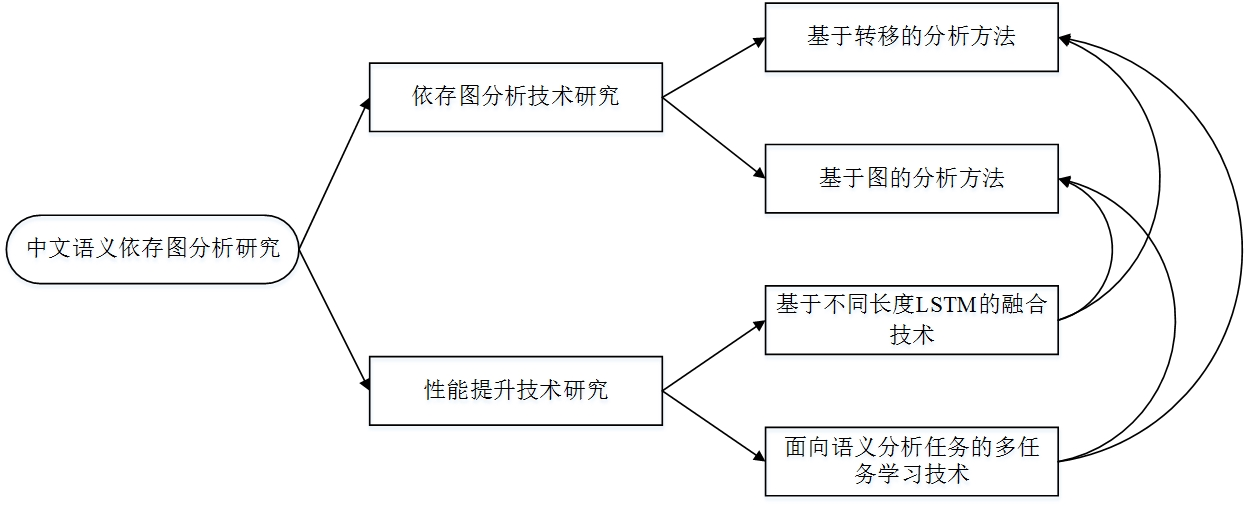
\includegraphics[width = 140mm]{picture/relation.jpg}
	\caption{研究内容概况图}
	\label{fig:relation}
\end{figure}



\subsection{实施方案}

由于四个研究点中的第一个已经完成,并且被录用,所以实施方案部分将主要介绍另外三个研究点。
研究工作将从如下几个方面展开:

\subsubsection{基于图的分析方法}

基于图的分析方法一般分为两步,第一步计算完全图中每个子结构的分数,第二步选出分数之和最大的子结构的组合作为预测出的目标结构。根据子结构的复杂度,基于图的分析模型可以分为一阶\citeyqy{mcdonald-crammer-pereira:2005:ACL}、二阶\citeyqy{mcdonald2006online}和高阶模型\citeyqy{koo-collins:2010:ACL},这里的阶数指的是每个子结构中依存弧的个数(例如一阶模型中每个子结构只包括一条弧)。高阶模型可以使用更复杂的子结构特征,因此其准确率更高,但解码算法的效率也会降低。

目前基于图的依存分析领域大部分工作的分析目标都是树结构的,由于依存树具有严格的结构限制(例如每个词只能有一个父节点),这些方法往往能够使用Eisner算法\citeyqy{eisner1996three}或在其基础上衍生出的其它动态规划算法\citeyqy{koo-collins:2010:ACL}进行解码。但是依存图结构中没有这些结构限制,因此上述方法在此不再适用。目前该方向的工作普遍采取了对每个子结构逐个判断的方法,这种方法虽然简单直观,但由于没有了结构限制,仅靠第一步计算的分数作为判断依据产生的依存图精度会受到很大影响。在此情况下要设计精度更高的基于图的依存分析方法,主要有两条路径,一是提高第一步中对每个子结构分数估计的准确性,二是选取更适合图结构的高阶模型,使得子结构本身就具有图的一定特性,从而提高最终得到的语义依存图的精度。接下来我们将分别介绍这两条路径的实施方案。

为了便于理解,我们首先以一阶模型为例,给出基于图的依存分析中第一步计算依存结构分数的形式化定义。在该模型中,一个依存结构的分数$s(\boldsymbol{x},\boldsymbol{y})$为其中所有子结构的分数之和(即所有弧的分数之和):

\begin{equation}
s(\boldsymbol{x},\boldsymbol{y})=\sum_{(i,j) \in \boldsymbol{y}} s(i,j)
\end{equation}

其中,$\boldsymbol{x}=x_1,\dots,x_n$表示输入句子,$\boldsymbol{y}$表示其对应的依存结构。我们可以将$\boldsymbol{y}$看作一个依存弧集合,因此$(i,j) \in \boldsymbol{y}$表示从词$x_i$指向词$x_j$的弧在$\boldsymbol{y}$中。

目前以依存图为分析目标的工作中,大多使用传统的基于离散特征的模型,使用高维稀疏的特征向量与特征权重向量的点积计算子结构的分值:

\begin{equation}
s(i,j) = \mathbf{w} \cdot \mathbf{f}(i,j)
\end{equation}

其中$\mathbf{f}(i,j)$表示从$x_i$指向$x_j$的弧对应的高维二元特征向量,$\mathbf{w}$表示特征权重向量。$\mathbf{f}(i,j)$中的每一维$f(i,j)$都用0和1表示一个特征是否出现,例如:

\begin{equation}
f(i,j)=
\begin{cases}
1& x_i = \text{"我" 且\ } x_j = \text{"是"} \\
0& \text{其他情况}
\end{cases}
\end{equation}

\citeayu{peng-thomson-smith:2017:Long}将依存句法分析领域中使用神经网络计算子结构分数的想法\citeyqy{kiperwasser2016simple}引入语义依存图分析中来,将句中词的词向量、词性向量作为双向LSTM的输入,然后将正向和反向LSTM的第$i$个时间节点的隐层状态拼接起来作为词$x_i$的表示向量$\mathbf{h}_i=[\overrightarrow{\mathbf{h}}_i;\overleftarrow{\mathbf{h}}_i]$。用这些低维致密的表示向量代替原有高维稀疏特征向量计算子结构分数,证明了该方法在依存图分析中的有效性。

\citeayu{peng-thomson-smith:2017:Long}的方法虽然成功将神经网络引入语义依存图分析任务中,但他们的对于词的表示比较单一,没有考虑一个词分别作为弧中的父节点和子节点时的不同情况。
目前基于图的句法分析方法中性能最好的是\citeayu{dozat2017deep}提出的基于深层双仿射(Biaffine)神经网络的分析器,他们凭借该分析器在CoNLL 2017多语言依存句法分析任务\citeyqy{zeman-EtAl:2017:K17-3}上取得了世界第一的成绩\citeyqy{dozat-qi-manning:2017:K17-3}。
该方法获得句中词的表示向量的步骤与\citeayu{peng-thomson-smith:2017:Long}相同,但在之后将这些表示输入4个不同的MLP分别获得每个词的4个表示向量:

\begin{equation}
\mathbf{h}^{(arc-dep)}_i = \text{MLP}^{(arc-dep)}(\mathbf{h}_i)
\end{equation}
\begin{equation}
\mathbf{h}^{(arc-head)}_i = \text{MLP}^{(arc-head)}(\mathbf{h}_i)
\end{equation}
\begin{equation}
\mathbf{h}^{(rel-dep)}_i = \text{MLP}^{(rel-dep)}(\mathbf{h}_i)
\end{equation}
\begin{equation}
\mathbf{h}^{(rel-head)}_i = \text{MLP}^{(rel-head)}(\mathbf{h}_i)
\end{equation}

其中$\mathbf{h}^{(arc-dep)}_i$和$\mathbf{h}^{(arc-head)}_i$分别表示$x_i$在计算弧的分数时作为子节点和作为父节点时的表示向量,$\mathbf{h}^{(rel-dep)}_i$和$\mathbf{h}^{(rel-head)}_i$分别表示$x_i$在计算弧标签分数时作为子节点和作为父节点时的表示向量。在此基础上利用双仿射分类器计算句中每个词作为词$x_i$的父节点时该弧的分数:

\begin{equation}
\begin{split}
\mathbf{s}^{(arc)}_i & = H^{(arc-head)}W^{(arc)}\mathbf{h}^{(arc-dep)}_i \\
& + H^{(arc-head)}\mathbf{b}^{\top(arc)}
\end{split}
\end{equation}

其中$\mathbf{s}^{(arc)}_i$是每个词作为$x_i$的父节点的分数向量,它的第$j$维表示弧$(j\rightarrow i)$的分数。$H^{(arc-head)} \in \mathbb{R}^{n \times d}$是句中$n$个词的$(arc-head)$表示向量拼接起来的矩阵。$W^{(arc)} \in \mathbb{R}^{d \times d}$是弧的权重矩阵,$\mathbf{h}^{(arc-dep)}_i$是词$x_i$的$(arc-dep)$表示向量,$\mathbf{b}^{(arc)}$是弧的偏移向量。使用这种方法,我们能够计算出任意两个词之间的弧的分数,在此基础上使用解码算法就能得到预测出的依存图结构。之后需要为每条弧计算出对应的弧标签,假设$y'_i$是我们预测出的词$x_i$的父节点,这条弧上弧标签的分数向量为:

\begin{equation}
\begin{split}
\mathbf{s}^{(rel)}_i & = \mathbf{h}_{y'^{(arc)}}^{\top(rel-head)}\mathbf{U}^{(rel)}\mathbf{h}^{(rel-dep)}_i \\
& + W^{(rel)}(\mathbf{h}^{(rel-dep)}_i \oplus \mathbf{h}^{(rel-head)}_{y'^{(arc)}_i}) \\
& + \mathbf{b}^{(rel)}
\end{split}
\end{equation}

其中$\mathbf{s}^{(rel)}_i \in \mathbb{R}^{k}$是$k$个弧标签的分数向量,每一维表示一个标签的分数。$\mathbf{h}_{y'^{(arc)}}^{(rel-head)}$是词$y'_i$的$(rel-head)$表示向量,$\mathbf{h}^{(rel-dep)}_i$是词$x_i$的$(rel-dep)$表示向量,$\mathbf{U}^{(rel)} \in \mathbb{R}^{d\times k \times d}$是弧标签的权重张量,$W^{(rel)} \in \mathbb{R}^{k \times 2d}$是弧标签的权重矩阵,$\mathbf{b}^{(rel)}$是弧标签的偏移向量。最终选择分数最高的弧标签作为这条弧上的标签$y'^{(rel)}_i$:

\begin{equation}
y'^{(rel)}_i = \arg \max_j s^{(rel)}_{ij}
\end{equation}

该方法不仅有效利用了神经网络强大的信息抽取能力,而且考虑了每个词作为弧中的父节点和子节点时的不同情况,因此在句法依存树分析任务中获得了目前最好结果。为了进一步提高基于图的语义依存图分析方法中第一步对每个子结构分数估计的准确性,我们会将该模型应用到依存图分析任务中来,为第二步的解码提供良好的基础。

\begin{figure}[hbtp]
	\centering
	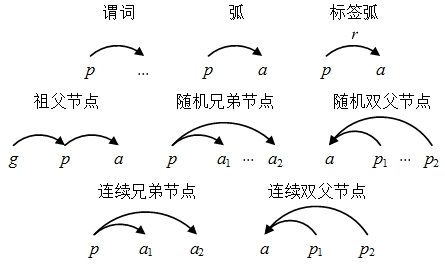
\includegraphics[width=100mm]{picture/parts.jpg}
	\caption{\citeayu{martins2014priberam}使用的子结构}
	\label{fig:parts}
\end{figure}

为了提高语义依存图分析的精度,我们还会尝试选取更适合图结构的高阶模型,使子结构具有图的一定特性。目前已有的基于图的语义依存图分析研究工作中,一般使用的是一阶或二阶模型。\citeayu{martins2014priberam}在其工作中首次使用了具有图特性的子结构,他们所使用的的所有子结构如图~\ref{fig:parts}所示。其中第一行三个为一阶分解,第二和第三行为二阶分解,随机双父节点和连续双父节点两种子结构为图结构所特有的。在依存句法分析领域,很多工作使用了超过二阶的模型,例如\citeayu{koo-collins:2010:ACL}和\citeayu{martins-almeida-smith:2013:Short}都使用了每个子结构包含三条弧的三阶模型。因此,我们将尝试将上述的随机双父节点和连续双父节点两种子结构扩展到三阶,即随机三父节点和连续三父节点,从而增强子结构的图特性,提高分析系统的精度。

\subsubsection{基于不同长度LSTM的模型融合技术}

模型融合技术目前已经在依存分析领域内取得了一些成功,被视为是一种简单而有效的提升系统性能的方式。但目前普遍被使用的模型融合技术要么是用不同的系统预测出的多个结果进行投票决定最终结果\citeyqy{du-EtAl:2015:SemEval},要么是在同一系统的训练中使用不同的随机初始化种子得到多个模型,然后在预测时同时使用这些模型\citeyqy{kuncoro-EtAl:2016:EMNLP2016,che-EtAl:2017:K17-3}。前者虽然有效且具有可解释性,但是要求设计多个不同且有效的分析系统,难度较大,往往被用于合并多个前人已经实现的系统。后者虽然只需要设计一个系统,但是可解释性不强。而且这两种方法都没有利用语义依存图的特性。

在语义依存图中,一个重要的区分依存弧的指标就是弧中两个词的距离。基于这一点观察,我们希望按照依存距离的不同建立多个模型,用它们分别对短、中、长距离的依存关系进行建模,然后对这些模型进行融合。因此,我们需要一个能够对可变长度序列进行编码的模型。

\begin{figure}[hbtp]
	\centering
	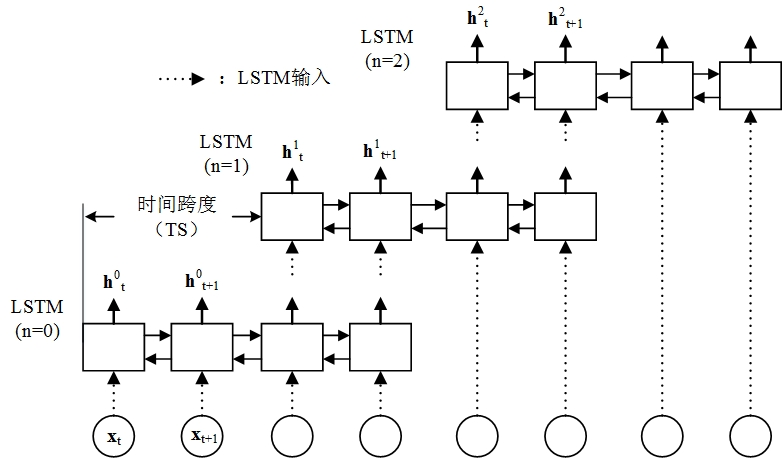
\includegraphics[width=130mm]{picture/ts-lstm.jpg}
	\caption{TS-LSTM网络结构示意图(LSTM个数$N=3$,窗口长度$W=4$,时间跨度$TS=2$)}
	\label{fig:ts-lstm}
\end{figure}

我们从\citeayu{lee2017ensemble}的动作识别的研究工作中得到了启发。他们提出了一种时间滑动长短时记忆网络(Temporal Sliding LSTM, TS-LSTM),由多个在输入序列上以一定的时间跨度滑动的LSTM组成。通过改变时间跨度$TS$和LSTM的窗口长度$W$可以实现提取不同长度依存信息的目的。该TS-LSTM的网络结构如图~\ref{fig:ts-lstm}所示。其中$x_t$表示句中第$t$个词的向量表示,

%该方法不但利用了语义依存图的结构特性,而且具有较强的可解释性,并且可以同时应用于基于转移的和基于图的分析方法中。

\subsubsection{面向语义分析任务的多任务学习技术}


\subsection{可行性分析}
\begin{enumerate}
	\item 本人长期关注自然语言处理相关技术、理论等。具有一定的理论基础,已经阅读并整理了大量的相关文献,对国内外研究现状有了较清晰的了解,详细掌握了目前中文语义依存图分析中存在的问题以及主要的研究方向。
	
	\item 我们的初期工作已经发表在CCL 2016,AAAI 2018等国内外重要学术会议上,其创新性得到了同行的认可。
	
	\item 所在的社会计算与信息检索研究中心经过多年的技术积累,已经基本掌握了自然语言处理中分词、词性标注、句法依存分析、语义角色标注等多种底层的关键技术。在上述各个方面都积累了大量的代码与数据,研究中心的语言技术平台享誉国内,加之本人对语义依存图分析技术已有较深刻的理解,这些技术和数据都为完成本课题提供了良好的支持。同时目前我实验室正在与北京语言大学合作完善中文语义依存图标注体系,标注更多中文语义依存图数据,这为本论文研究工作的开展起到了很大的帮助。
	
	
\end{enumerate}
\section{论文的进度安排与预期目标}

\subsection{进度安排}

2016年9月 - 2017年3月:博士论文选题,参考文献收集。

2017年4月 - 2017年10月:完成基于转移的语义依存图分析方法研究,完成论文写作并发表

2017年11月 - 2018年6月:完成针对语义依存图特点的模型融合技术的研究

2018年7月 - 2019年4月:完成基于图的语义依存图分析方法研究

2019年5月 - 2019年12月:完成利用多语言、多领域数据帮助中文语义依存图分析的研究

2020年1月 - 2020年6月:撰写毕业论文,申请毕业答辩。


\subsection{预期目标}

本课题致力于解决中文语义依存图分析中的关键问题,其中包括两部分,首先是语义依存图分析方法本身,然后是如何提高这些方法的性能。在前期的探索中,我们利用基于转移的依存分析方法,提出了新的能够分析语义依存图的转移系统,同时设计了新的网络结构,利用LSTM获取转移状态的信息用于转移动作的预测。这部分工作已经在中文语义依存图问题上取得了目前最好的结果,下一步的工作,我们要沿着依存分析的另一条道路,探索基于图的语义依存图分析方法。同时还要在这两类方法的基础上研究针对语义依存图特点的模型融合技术以及如何利用多语言、多领域数据帮助语义依存图分析。综合这些工作,我们预期目标为分别利用基于转移和基于图的方法解决中文语义依存图分析问题,利用多项技术提高这些方法的性能,并比较两类方法在该问题上的优劣,最终构建一个高效且能够利用更丰富的资源的实用的中文语义依存图分析系统。

\section{学位论文预期创新点}
与前人已发表的研究成果相比,本学位论文的预期创新点主要有以下几点:

(1)提出了一个利用注意力机制来直接生成顺滑块的方法。传统的序列标注等方法很难充分的利用全局信息,而我们的基于注意力机制的方法首先会对整个句子进行编码,之后再次序的生成顺滑块,其可以理解为一个全局的决策过程,因此能够充分的利用全局信息。

(2)提出了一个基于转移的顺滑方案。顺滑任务的一个主要的特点是非顺滑块和对应的顺滑块之间有很强的相似性,我们设计的基于转移的方案可以很好的利用这些块之间联系,实验结果表明基于转移的方案取得了目前最好的试验效果。

(3)正在实现的基于easy-first的顺滑方案。以前的方案大都是从左往右进行决策,这种方案的主要问题是决策是局部的,而且只能看到很少的右边的信息。我们设计的基于easy-first的方案的生成过程是一个由易到难的过程,避开了从左往右进行决策的问题,而且我们的方案在决策的过程中还能充分的利用块信息。

(4)正在实现的基于dual learning的顺滑方案。以前的方案大部分只关注模型本身的改进,很少有利用大量未标注数据的方案。我们的方案通过正向和逆向两个模型的互相交互,将大量的口语数据和标准的新闻数据引入进来,从而期望能利用更少的语料,取得不错的实验效果。


\section{为完成课题已具备和所需的条件、外协计划及经费}
\begin{enumerate}
	\item 相关工作的理论基础的积累:包括文献整理、平台搭建等工作(已完成);
	\item 基于注意力机制的顺滑方案:首次从生成的角度来解决顺滑问题(已完成);
	\item 基于转移的顺滑方案:该方案可以充分的利用不同块之间的信息(已完成);
	\item 基于easy-first的方案:已完成初步的方案设计和代码编写,进一步的实验结果即将得出;
	\item 基于dual learning的方案:已完成初步的方案设计,即将开始编写代码;
	\item 本论文的课题研究经费充足,能够保证相关工作正常进行。
	\item 本论文的课题研究得到了科大讯飞公司合肥研究院(总部)的鼎力支持。
\end{enumerate}


\section{预计研究过程中可能遇到的困难、问题,以及解决的途径}

\begin{enumerate}
	\item 在dual learning方案中如何约束逆向的生成过程:对于dual learning方案,逆向的生成过程是由顺滑的(不含不流畅块)句子生成含有不流畅块的句子,在理论上,在顺滑句子的基础上添加任何成分都是合理的,但是这样无限制的生成方案可能会带来严重的问题,也就是说正向和逆向不是严格对称的,因此如何消除或者减少这种不对称将是实验过程中需要重点关注的部分。
	\item 训练语料不足问题:由于复杂的神经网络需要大规模的训练语料,现有的English SwitchBoard数据只有八万句左右,当模型变复杂的时候,其规模略小。由于实验室跟讯飞有相关的合作,讯飞方面将负责标注大量的中文语料,从而能很好的验证我们模型在大规模语料上的效果。
	\item 实验结果不理想的问题:实验效果不理想可能是由多种不同的原因造成的。如果遇到这种问题,首先会排查代码是否有bug。其次,会对实验结果进行详细的分析,进而根据实验结果,决定是否对模型进行调整和优化。
\end{enumerate}

\section{发表论文情况}
\begin{enumerate}
	\item \textbf{Yuxuan Wang}, Wanxiang Che, Jiang Guo and Ting Liu. A Neural Transition-Based Approach for Semantic Dependency Graph Parsing. In Proceedings of the 32nd AAAI Conference on Artificial Intelligence (AAAI 2018). 2018.02. New Orleans, LA, USA.(已录用, CCF排名A类,重要国际会议,oral)
	\item \textbf{Yuxuan Wang}, Jiang Guo,  Wanxiang Che, and Ting Liu. Transition-Based Chinese Semantic Dependency Graph Parsing. In Proceedings of China National Conference on Chinese Computational Linguistics (CCL 2016,最佳论文奖,oral). 2016.10. Yantai, China.
\end{enumerate}

\clearpage

\newpage


\bibliographystyle{GBT7714-2005NLang-HIT}
\addtolength{\bibsep}{-0.8em}
\nocite{*}
\bibliography{reference}

\end{document}
